%%
% 今時jarticleやjbook使ってる人いる?時代はjsarticleかjsbookだよ
% ついでに言うと、uplatexってのはplatexの上位互換、これを使わないなんて旧世代だよね
%
\documentclass[uplatex, report, a4j, 10pt]{jsbook}

\usepackage{packages/miyazaki-u-paper}   % 宮崎大学工学部の卒論の基本(片山先生作)を、僕がちょっと書き換えちゃった(テヘッ
\usepackage{enumitem}           % enumerate?古い古い
\usepackage[dvipdfmx]{graphicx} % 当然dvipdfmなんて使ってないよね
\usepackage[dvipdfmx]{color}    % listingsを使うときにはこれも必須、dvipdfmxを変えちゃうとgraphicxのdvipdfmxも変わるよ
\usepackage{listings, packages/jlisting} % コードを埋め込むなら必須
\usepackage{txfonts}            % フォントといえばやっぱりtxfonts、今はnewtxってのもあるらしい
\usepackage{verbatim}           % コメントアウトしてくれる便利なプリアンブルが使える \begin{comment} ... \end{comment}
\usepackage{url}
% \usepackage{easy-todo}
\usepackage[hdivide={21mm, , 21mm}, vdivide={30mm, , 25mm}]{geometry} % スタイルを少し変えたくても\hoffset, \voffsetは使わないでね
\usepackage{multirow}
\usepackage{ascmac}
\usepackage{subcaption}
\usepackage{colortbl}
\usepackage[dvipdfmx, hidelinks]{hyperref} % リンクを付けてくれる。
\usepackage{pxjahyper}          % リンクを付けてくれる(日本語)

% ソースコードの設定
\lstset{
  breaklines = true,%自動で折り返す
  basicstyle={\footnotesize\ttfamily},
  numberstyle={\scriptsize},
  stepnumber=1,
  numbersep=1zw,
  lineskip=-0.5ex,
  frame=single,
  numbers=left,%行番号を左に
  framexleftmargin=6mm,%行番号をフレーム内に
  numberstyle=\scriptsize,%行番号のサイズ
  stepnumber=1%1行おきに行番号を
}

% \addtolength\oddsidemargin{-1.5zw}  % 魔法の呪文01
% \addtolength\evensidemargin{-1.5zw} % 魔法の呪文02
% \addtolength\textwidth{3.0zw}       % 魔法の呪文03

\setcounter{page}{1}
\newcommand{\ttt}[1]{\texttt{#1}}
\newcommand{\ift}{if-then-else}
% \newcommand{\toolName}{AWSETIL}  % ツール名を設定

%%
% miyazaki-u-paper.sty用設定値
%
% \degree{g} % Graduateのg or Masterのm
% \figurenumbering{f} % 図目次を付ける場合はt (真) を持つ真偽値を引数に取る関数
% \tablenumbering{f} % 表目次を付ける場合はt (真) を持つ真偽値を引数に取る関数
\title{電子フォーム作成時間の削減を目的とした\\ラベル付き記入欄検出手法の提案\\}
\author{木村 優哉}
\nendo{5} % 年度
\advisor{片山 徹郎 教授} % 修論では無視する
\major{情報システム工学科}


\begin{document}
\maketitle

% \setlength\textfloatsep{0pt}% 魔法の呪文04

%
% 概要
%
\preface{概要}
作成予定

%
% 本文
%
\chapter{はじめに}\label{cha:Introduction}
2019年4月に電子帳簿保存法が改正され、帳簿書類の電子データ保存が義務付けられたことにより、帳簿書類の電子化が推進されている\cite{電子帳簿保存法}。
また、総務省の令和2年版「情報通信白書」では、60.4\%の企業が社内業務のペーパーレス化に取り組んでいると答えた\cite{デジタルデータの経済的価値の計測と活用の現状に関する調査研究}。
しかし、Biz Clipによる文書管理実態調査2023によると、紙の文書が介在する業務工程のうち、契約・申請書類は、2020年時点で2023年時点で66.5\%、2023年で59.1\%であるという結果となり、特に契約書や請求書といった帳票は、比較的に紙媒体が多いことがわかった\cite{文書管理実態調査2023}。

帳票の電子化は、スキャナや写真などで帳票を撮影することで実現できる。
しかし、帳票に記入した内容は、人が目視で確認する必要がある。
効率的に記入内容を管理するためには、その記入内容をデータとして保存する必要がある。
その方法の1つとして、電子フォームを用いる方法がある。
電子フォームとは、従来紙の帳票で行っていた申請などの業務を電子化し、アプリケーションを介して入力した項目をそのまま業務用のデータとして利用するための仕組みである\cite{電子フォーム}。
電子フォームを用いることで、記入内容をデータとして保存することができる。
しかし、電子フォームを作成するには、以下の2つの課題がある。

\begin{itemize}
  \item 電子フォームの作成に時間がかかる
  \item 使い慣れた既存の帳票のレイアウトが変更となる場合がある
\end{itemize}

これらの課題を解決するため、電子フォームを自動作成するツールやサービスがある。
既存の電子フォーム作成ツール\cite{i-Reporter}\cite{Create!Form}は、Excelファイルを入力とすることにより、記入欄の位置を取得することができ、セルに設定した書式設定を保持した状態で、電子フォームを自動で作成できる。
しかし、Excelファイルを入力とした場合は、レイアウトが変更となる可能性がある。
また、画像ファイルを入力とした場合は、入力する画像を背景とするため、レイアウトは変更とならないが、マウス操作で記入欄を配置する必要があるため、手間と時間がかかる。
さらに、書式についての情報がないため、記入欄に書式の設定をすることができない。

そこで本研究は、前述した2つの課題点を同時に解決するため、帳票画像内における記入欄の領域座標、および、その記入欄に入力する内容のデータ型をまとめたJSONファイルに加えて、検知した記入欄を強調表示した画像2枚を出力する、記入欄の検出およびラベル付与手法を提案する。
まず、帳票画像内にある記入欄の位置を取得するために、記入欄を画像処理によって検出する。
次に、検出した記入欄に入力する内容のデータ型を決定するために、入力内容を示す文字を認識し、大規模言語モデルを用いて、記入する内容が、日付(date)、文字列(string)、数値(number)の3種類のうちいずれかを、ラベルとして割り付ける。
そして、取得した記入欄の領域座標を参照して、帳票画像に色を付けて描画することで、取得した記入欄を強調表示した画像を出力する。
記入欄の検出およびラベル付与手法の提案を実現するための手段として、これらの処理を行うツールを作成する。

本論文の構成を、以下に示す。\\
第2章では、本研究に必要となる前提知識について説明する。\\
第3章では、本ツールの持つ機能について説明する。\\
第4章では、本ツールの実装について説明する。\\
第5章では、本ツールの適用例について説明する。\\
第6章では、本ツールについて考察する。\\
第7章では、本研究のまとめと今後の課題を示す。
\chapter{研究の準備}\label{cha:Preparation}
(簡単なメモ。途中まで記述。あとで詳しく書くこと)

本章では、本研究に必要な前提知識について説明する。


\section{入力対象の画像}\label{sec:input_images}
本提案手法の入力対象である画像については、以下の条件を全て満たす画像とする。
なお、帳票は帳簿と伝票の総称であり\cite{帳票}、電子文書は、Wordやテキストファイルなど、デジタル情報として作成した文書を指し、電子化文書は紙媒体の書類をスキャンしたPDFファイルや画像などの形式で保存した文書を指す\cite{電子文書と電子化文書}。
電子化文書については、本提案手法においては、スマートフォンのカメラで撮影した帳票を想定する。

\begin{itemize}
	\item 帳票の電子文書または電子化文書の画像である。
	\item 帳票の背景が白色である。
	\item 日本語かつ横書きの帳票である。
	\item 文字が手書きではない。
	\item 入力欄が矩形または下線で示されている。
\end{itemize}

なお、入力対象とする画像の座標系は、画像左上隅画素を原点(0,0)とし、右方向をX軸の正の向き、下方向をY軸の正の向きと定義する。

\section{バリデーションチェック}\label{sec:validation_check}


\section{OpenCV}\label{sec:OpenCV}
OpenCV(Open Source Computer Vision Library) は、コンピュータビジョン向けのオープンソースライブラリである\cite{OpenCV}。
本研究では、OpenCVに用意されている以下の関数を用いる。

\paragraph{imread関数}
imread関数は、画像ファイルを読み込む関数である。

\paragraph{cvtColor関数}
cvtColor関数は、画像の色空間を変換する関数である。
本研究では、読み込んだ画像をグレースケール化するために用いる。
これは、カラー画像をグレースケール化することにより、画像処理に必要な計算量を減らす目的がある。

\paragraph{getStructuringElement関数}
getStructuringElement関数は、カーネルを作成する関数である。
カーネルは、ガウシアンフィルタ(GaussianBlur関数で後述)や膨張処理(dilate関数で後述)など、注目画素の周囲の画素値を参照する画像処理において、周囲の画素を行列として、周囲の画素を参照する計算に付ける重みである。
例えば、3行3列のカーネルは、注目画素とその周囲8画素の画素値の、計9画素の画素値を用いて計算を行う。
第一引数として、カーネルの形状を矩形、楕円、十字から決定する。
また、第二引数では、カーネルの大きさを指定する。
本研究では、矩形領域座標取得用画像処理(\ref{subsec:image_processing_for_rect_coords_obtainment}節で後述)に必要な画像処理の一部として用いる。

\paragraph{GaussianBlur関数}
GaussianBlur関数は、ガウシアンフィルタを適用することにより、画像内の白色ノイズを除去する関数である。
ガウシアンフィルタは、注目画素との距離に応じて重みを変えるガウシアンカーネルを用いた、画像の平滑化によって白色ノイズを除去するフィルタである。
標準偏差を$0$とするによって、カーネルの大きさから自動的に標準偏差を計算する\cite{ガウシアンフィルタ}。
本研究では、矩形領域座標取得用画像処理(\ref{subsec:image_processing_for_rect_coords_obtainment}節で後述)に必要な画像処理の一部として用いる。

\paragraph{threshold関数}
threshold関数は、画像を二値化する関数である。
第一引数として、グレースケール画像を指定する。
また、第二引数では、二値化する際の閾値を指定し、第三引数では、二値化後の画素値の最大値を指定する。
さらに、第四引数では、二値化における閾値処理手法を指定する。
本研究で用いる閾値処理手法を指定する変数を、以下に示す。

\begin{itemize}
	\item THRESH\_BINARY\\
		文字情報取得用画像処理(\ref{subsec:image_processing_for_char_recognition}節で後述)で設定する。
		大津の二値化\cite{大津の二値化}を用いる場合は、大津の二値化によって決定した閾値を基準に、ある注目画素の画素値が閾値よりも小さい場合は画素値を第三引数で設定する値に変換し、閾値よりも大きい場合は画素数を0に変換して二値化する。
	\item THRESH\_BINARY\_INV\\
		下線部領域座標取得用画像処理(\ref{subsec:image_processing_for_underline_coords_obtainment}節で後述)で設定する。
		大津の二値化を用いる場合は、大津の二値化によって決定した閾値を基準に、ある注目画素の画素値が閾値よりも小さい場合は画素値を0に、閾値よりも大きい場合は画素値を第三引数で設定する値に変換して二値化する。
	\item THRESH\_TOZERO\_INV\\
		矩形領域座標取得用画像処理(\ref{subsec:image_processing_for_rect_coords_obtainment}節で後述)で設定する。
		大津の二値化を用いる場合は、大津の二値化によって決定した閾値を基準に、ある注目画素の画素値が閾値よりも小さい場合は画素値を変換せず、閾値よりも大きい場合は画素値を第三引数で設定する値に変換して二値化する。
\end{itemize}

大津の二値化(判別分析法)は、画素値のヒストグラムにおけるクラス間分散とクラス内分散の比である分離度が最大となる閾値を求める手法である\cite{大津の二値化}。
大津の二値化を用いることによって、画像に適する閾値を自動で決定することができる。
大津の二値化による閾値処理を設定する場合は、第四引数に、変数THRESH\_OTSUを加算演算子+で接続する。
なお、一般に8ビット画像について、画素値は0に近づくほど黒を、255に近づくほど白を表すとされている\cite{画素値}。
本研究では、大津の二値化を用いて、閾値を決定する。

\paragraph{dilate関数}
dilate関数は、画像に膨張処理を施す関数である。
膨張処理は、ある注目画素について、一定周囲の画素集合内に白色に二値化した画素がある場合は、注目画素の画素値をカーネル内画素の最大画素値に変更する処理である\cite{膨張処理}。
第一引数として、二値化処理後の画像である、二値画像を指定する。
また、第二引数では、カーネルを指定する。
さらに、第三引数では、膨張処理を適用する回数を指定する。
本研究では、矩形領域座標取得用画像処理(\ref{subsec:image_processing_for_rect_coords_obtainment}節で後述)で施す画像処理のひとつとして用いる。

\paragraph{Canny関数}
Canny関数は、Canny法によってエッジ検出を行う関数である。
エッジ検出は、画像内の輝度差を検出することにより、物体や領域の境界を識別する処理である\cite{エッジ検出}。
Canny法は、ガウシアンフィルタでノイズを除去し、ソーベルフィルタでエッジの勾配と方向を検出し、エッジを細線化した後に勾配と方向からエッジ検出を行う手法である。
Canny法におけるエッジ検出の閾値処理については、最低閾値と最大閾値を決め、画素値の微分値が最大閾値よりも大きい画素と、それらに隣接しており、かつ最低閾値よりも大きく最大閾値よりも小さい画素のみをエッジとみなすヒステリシス閾値処理を用いる\cite{Canny法}。
本研究では、下線部領域座標取得用画像処理(\ref{subsec:image_processing_for_underline_coords_obtainment}節で後述)で下線部領域座標の取得に必要な画像処理の一部として用いる。

\paragraph{findContours関数}
findContours関数は、画像内にある物体の輪郭を検出する関数である。
第一引数として、二値化処理後の画像である二値画像を指定する。
また、第二引数では、検出する輪郭と、それらを保存する構造を決定する変数を指定する。
本研究では、全ての輪郭を検出し、それらを外側から順に入れ子とした階層構造とするRECT\_TREEを指定する。
さらに、第三引数では、輪郭となる頂点の近似法を決定する変数を指定する。
本研究では、輪郭を表現するにあたり、冗長な点の情報を削除するCHAIN\_APPROX\_SIMPLEを用いる。
例えば、矩形であれば、各辺にある全ての点の座標を保存する必要はなく、4つの頂点の座標を保存することで、矩形の輪郭を表現できるため、それ以外の座標情報を削除する\cite{輪郭検出}。
本研究では、矩形領域座標取得処理(\ref{subsec:rect_coords_obtainment_processing}節で後述)で矩形の輪郭を検出するために用いる。

\paragraph{HoughLinesP関数}
HoughLinesP関数は、ハフ変換によって画像内にある直線を検出する関数である。
ハフ変換は、二値画像中の直線や円を検出する手法の1つであり、画像空間から$\rho$-$\theta$空間に、座標系を変換することで、直線や円を検出する手法である。
直線を検出する場合は、極座標の二次元平面に変換する。
直線上のある点の座標を$(x, y)$とすると、$\rho$は、座標$(x, y)$を通る直線に対して、原点から垂線を下ろしたときの長さ、$\theta$は、座標$(x, y)$を通る直線に対して、原点から垂線を下ろしたときに、X軸となす角度と表すことができる。
よって、以下の式が成り立つ。

\begin{equation}\label{eq:hough}
	\rho = x\cos\theta + y\sin\theta
\end{equation}

座標$(x, y)$を通る直線は無数に存在するため、式\ref{eq:hough}を満たす$(\rho, \theta)$も無数に存在する。
縦軸を$\rho$、横軸を$\theta$として、それらの$(\rho, \theta)$を、$\rho$-$\theta$空間に射影すると、線を図示できる。
この座標系の変換を、直線上の他にある$(x, y)$以外の座標に対して行ったとき、$\rho$-$\theta$空間に交点が存在する。
この操作を全画素に対して行い、$\rho$-$\theta$空間で多くの線が重なっている点$(\rho, \theta)$から、直線が存在する可能性が高い$(\rho, \theta)$を探し、直線を検出する\cite{ハフ変換}。
HoughLinesP関数を用いる際は、以下の順で引数を渡す\cite{HoughLinesP関数の引数}。
\begin{enumerate}
	\item 直線を検出する二値画像のパス
	\item 式\ref{eq:hough}における、$\rho$の値
	\item 式\ref{eq:hough}における、$\theta$の値
	\item 直線とみなす集合した点の数の閾値
	\item 直線とみなす最小の長さ
	\item 同一直線とみなす2つの点の間隔の広さ
\end{enumerate}
本研究では、下線部領域座標取得処理(\ref{subsec:underline_coords_obtainment_processing}節で後述)で直線を検出するために用いる。

\paragraph{drawContours関数}
drawContours関数は、輪郭を画像に描画する関数である。
drawContours関数を用いる際は、以下の順で引数を渡す\cite{輪郭描画}。
\begin{enumerate}
	\item 輪郭を描画する画像のパス
	\item 描画する輪郭のリスト
	\item 第二引数のうち、描画する輪郭のインデックス($-1$を指定することで、全輪郭を描画する)
	\item 輪郭を描画する線のRGBカラーを示すタプル
	\item 輪郭を描画する線の太さ
\end{enumerate}
本研究では、文字情報取得用画像処理(\ref{subsec:image_processing_for_char_recognition}節で後述)で白色の矩形と直線を描画するためと、領域強調画像出力処理(\ref{subsec:area_highlighted_image_output_processing}節で後述)で矩形領域と下線部領域を描画するために用いる。

\paragraph{putText関数}
putText関数は、文字を画像に描画する関数である。
本研究では、領域強調画像出力処理(\ref{subsec:area_highlighted_image_output_processing}節で後述)で領域とラベルを描画するために用いる。

\section{DeblurGANv2}\label{sec:DeblurGANv2}
DeblurGANv2は、敵対的生成ネットワーク(GAN)をブレ除去に適用したツールである\cite{DeblurGANv2}。
スマートフォンで帳票画像を撮影する際に発生する画像内のブレを除去し、領域座標と文字認識の精度を高めることを目的として適用する。
また、先行研究において、スマートフォンのカメラで撮影した画像に対して、複数の画像処理と共にDeblurGANv2を適用することによって、ブレ除去によって画像品質が向上し、Tesseract-OCR\cite{Tesseract-OCR}を用いた光学文字認識(\ref{sec:Optical-Charactor-Recognition}節で後述)の精度が向上することが示されている\cite{DeblurGANv2の先行研究}。
本研究では、領域取得部(\ref{sec:area_coords_obtainment_part}節で後述)と文字情報取得部(\ref{sec:OCR_part}節で後述)で施す画像処理の1つとして用いる。


\section{光学文字認識}\label{sec:Optical-Charactor-Recognition}
光学文字認識(Optical Charactor Recognition)とは、文字を含む画像から文字コードに変換することである\cite{光学文字認識}。
本研究では、文字情報取得処理(\ref{subsec:char_recognition_processing}節で後述)および文字位置取得処理(\ref{subsec:char_information_obtainment_processing}節で後述)で、文字と、文字を囲むバウンディングボックスの各頂点のxy座標を取得するために用いる。
また、本研究では、光学文字認識ソフトウェア\cite{光学文字認識ソフトウェア}であるTesseract-OCRを、PythonのOCR用のラッパーライブラリであるPyOCR\cite{PyOCR}から用いる。
PyOCRを用いることにより、文字を認識する処理にbuilderという変数をパラメータとして指定できる。
本研究では、LineBoxBuilderを変数builderに指定し、行単位で文字と、文字を囲むバウンディングボックスの各頂点のxy座標を同時に取得する。

\section{Fugashi}\label{sec:Fugashi}
Fugashiは、形態素解析ソフトウェアであるMecab\cite{Mecab}をPython\cite{Python}で使用する際のラッパーライブラリである\cite{Fugashi}。
本研究では、除外判定処理(\ref{subsec:exclusion_judgement_processing}節で後述)で属性判定に不要な取得文字を、取得文字を構成する形態素の品詞を参照することによって、出力の対象外とするために用いる。
また、本研究でFugashiの解析に用いる辞書として、UniDic\cite{UniDic}を利用する。
よって、本論文で記述する品詞体系についてはUniDic品詞体系とする。
UniDic品詞体系では、左からカンマ区切りで、大分類、中分類、小分類、細分類の順で品詞を列挙する\cite{UniDic品詞体系}。


\section{Youri}\label{sec:Youri}
Youriは、Llama2\cite{Llama2}を日本語の学習データで継続事前学習を行うことによって、日本語のテキスト生成能力を高めた大規模言語モデルである\cite{Youri}。
本研究では、属性推測処理(\ref{subsec:att_prediction_processing}節で後述)で取得文字の属性を判定するために用いる。
\chapter{本提案手法の機能}\label{cha:Function}
本研究では、帳票画像内の記入欄である領域の座標を取得後、文字の属性を判定し、取得文字近傍に存在する記入欄の座標に対してラベルを割り当て、領域の座標と、対応するラベルを組とするJSON形式のファイルを出力する手法を提案する。

本章では、本研究で提案する帳票画像内の記入欄を自動検出する手法の機能について説明する。
本提案手法は、\ref{sec:input_images}節で述べた帳票画像を入力とする。
出力は、領域の座標と、対応するラベルを組とするJSON(JavaScript Object Notation)形式のファイルと、領域の座標を帳票画像に描画したPNG(Portable Network Graphics)形式の画像である。
出力する画像については、矩形の領域を描画した画像と、下線部の領域を描画した画像の2枚に分けている。
これは、領域の誤検出によって、描画した矩形と直線が重なった場合、視認性が低下することを防ぐためである。
なお、本研究において、以下の名称を用いる。

\begin{itemize}
    \item 帳票画像記入欄\\
          入力である帳票画像内の記入欄。
    \item 電子フォーム記入欄\\
          本提案手法によって取得した座標で示す記入欄。
    \item 矩形領域\\
          電子フォーム記入欄のうち、矩形で示された記入欄。
    \item 下線部領域\\
          電子フォーム記入欄のうち、直線で示された記入欄。
    \item 領域座標\\
          本提案手法によって取得する領域の座標。
          矩形領域であれば、各頂点のxy座標にあたる。
          下線部領域であれば、両端点のxy座標にあたる。
    \item 文字情報\\
          文字認識によって得る、認識した文字と、それを囲むバウンディングボックスの各頂点のxy座標。
    \item 属性\\
          文字認識によって得た文字から推測するデータ型。
    \item ラベル\\
          文字の近傍に存在する電子フォーム記入欄に対して、文字位置と属性から推測するデータ型。
\end{itemize}

また、本研究で提案する手法は、以下の2つの機能を持つ。

\begin{itemize}
    \item ラベル付き領域座標取得機能
    \item 領域描画画像出力機能
\end{itemize}

本提案手法の入力対象である帳票画像を例として、図\ref{fig:original}に示す。
また、図\ref{fig:original}に対して、本提案手法を適用し、出力したJSONファイルの一部を、図\ref{fig:example_output_json}に示す。
出力するJSONファイルは、配列rects\_dataと、配列underlines\_dataで構成し、矩形領域の情報、下線部領域の情報をそれぞれ持つ。
これら2つの配列は、それぞれ以下の情報をもつ。

\begin{itemize}
    \item 配列ごとに一意であるid
    \item 領域に割り付けているラベルを示すlabel
    \item 領域座標を示すオブジェクトcoords
\end{itemize}

\begin{figure}[t]
    \begin{center}
        \fbox{
            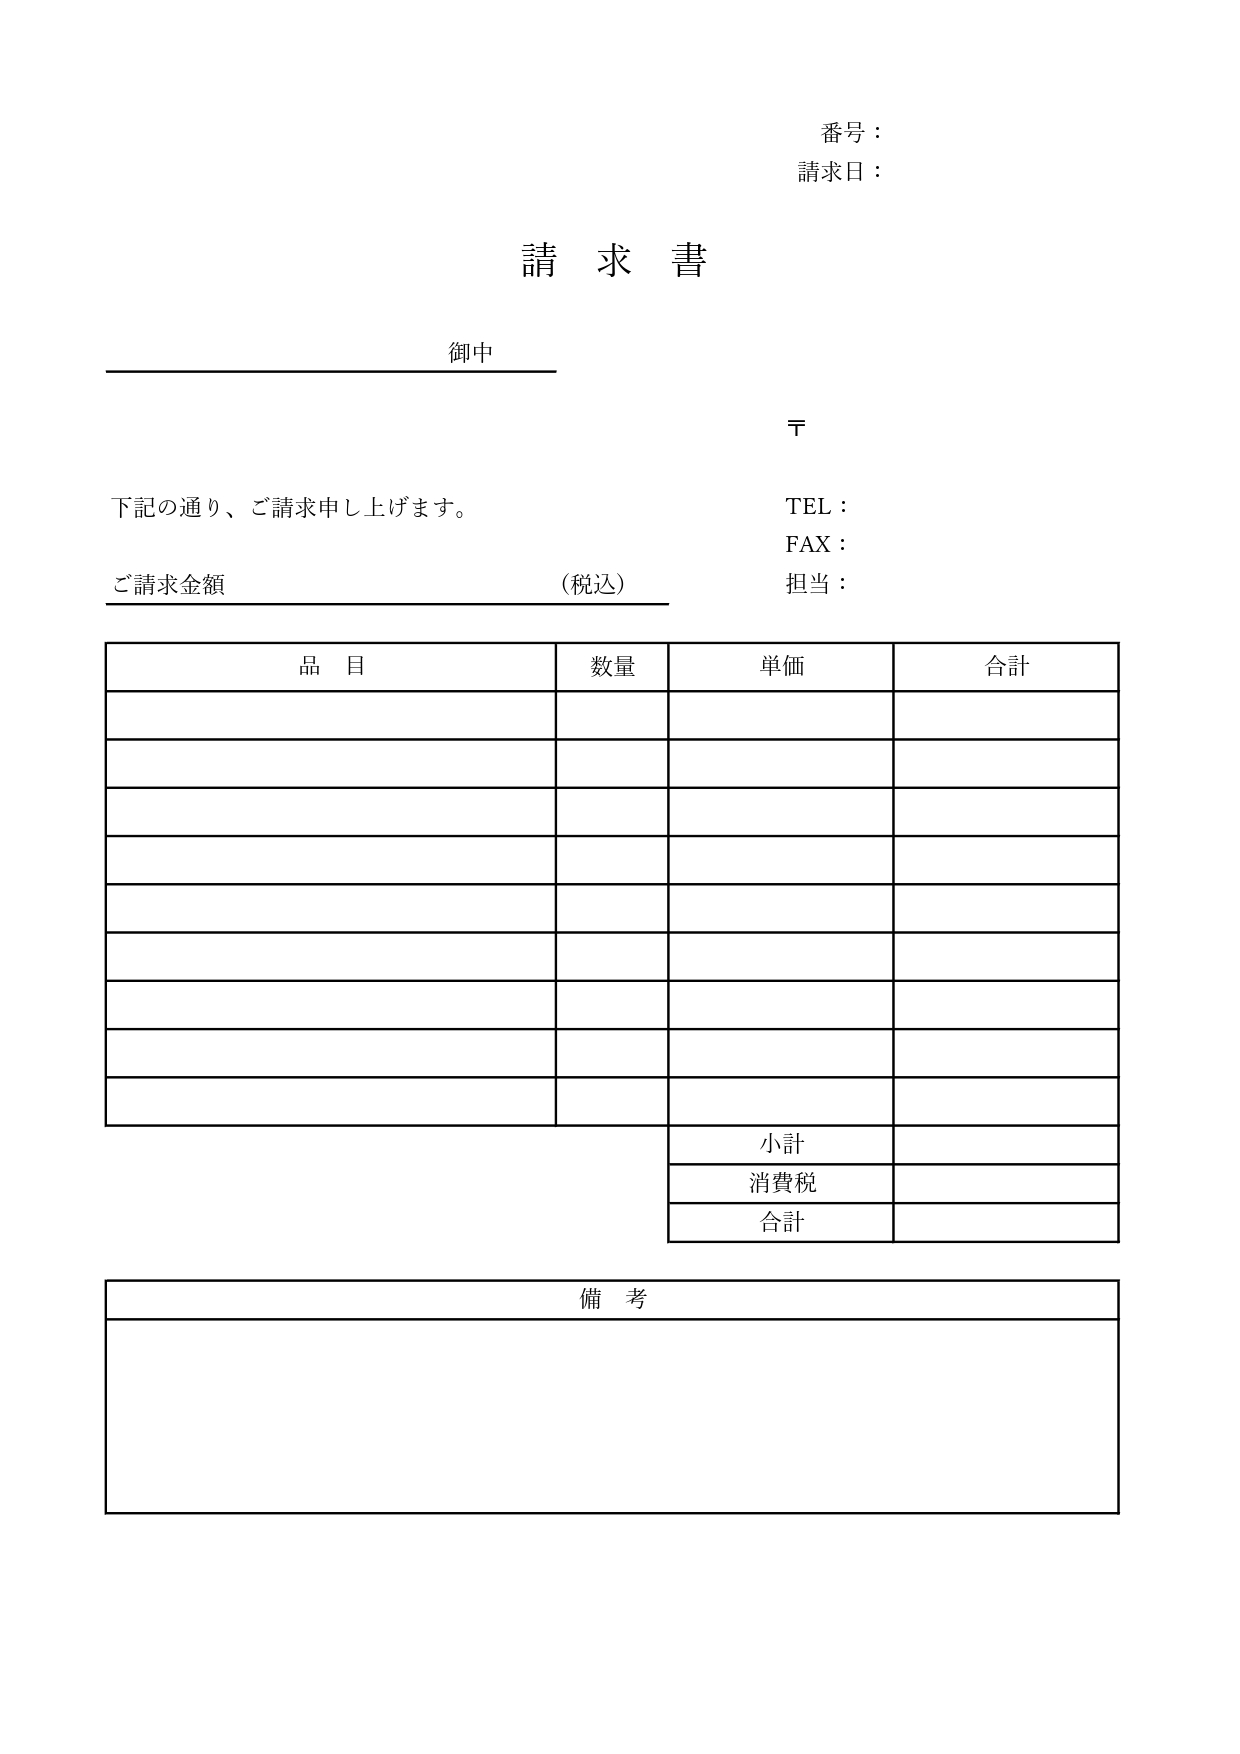
\includegraphics[width=15cm]{image/03-function/original.jpg}
        }
        \caption{入力対象である帳票画像の例}
        \label{fig:original}
    \end{center}
\end{figure}


\lstset{language=}
\begin{figure}[t]
    \begin{lstlisting}
{
    "rects_data": [
        "id": 0, 
        "label": "number",
        "coords": {
            "top_left": {
                "x": 1339,
                "y": 1288
            },
            "buttom_left": {
                "x": 1339,
                "y": 1377
            },
            "buttom_right": {
                "x": 1782,
                "y": 1377
            },
            "top_right": {
                "x": 1782,
                "y": 1288
            }
        }
    ],
    "underlines_data": [
        "id": 0,
        "label": "string",
        "coords": {
            "left": {
                "x": 213,
                "y": 742
                },
            "right": {
                "x": 1111,
                "y": 742
            }
        }
    ]
}
    \end{lstlisting}
    \caption{出力するJSONファイルの一部}\label{fig:example_output_json}
\end{figure}

\section{ラベル付き領域座標取得機能}\label{sec:eform_write_space_obtainment_feature}
ラベル付き領域座標取得機能は、取得対象の記入欄である矩形の領域および下線部の領域について、各領域の座標を電子フォーム記入欄として取得する機能である。
電子フォーム記入欄にラベルを割り付けることにより、バリデーションチェック(\ref{sec:validation_check}節を参照)に必要な情報を付与することができる。

電子フォーム記入欄の取得は、以下の手順で行う。

\begin{enumerate}
    \item 矩形領域取得
    \item 下線部領域取得
    \item 文字情報取得
    \item 属性推測
    \item ラベル割付
\end{enumerate}

\subsection{矩形領域取得}\label{subsec:rect_coords_obtainment}
矩形領域取得は、矩形の領域を帳票画像記入欄とみなし、各頂点のxy座標を領域座標として取得する。
以降、下線部の領域座標と区別するため、矩形領域の領域座標を、矩形領域座標と呼ぶ。
取得した矩形領域座標を、y座標について昇順にソートし、0から順に番号を割り振る。
出力するJSONファイルにおける、rects\_data配列内の、idキーに対応する値とcoordsオブジェクトのデータを取得する。

\subsection{下線部領域取得}\label{subsec:underline_coords_obtainment}
下線部領域取得は、水平な直線を帳票画像記入欄とみなし、両端点のxy座標を領域座標として取得する。
以降、矩形の領域座標と区別するため、下線部領域の領域座標を、下線部領域座標と呼ぶ。
取得した下線部領域座標を、y座標について昇順にソートし、0から順に番号を割り振る。
出力するJSONファイルにおける、underlines\_data配列内の、idキーに対応する値とcoordsオブジェクトのデータを取得する。

\subsection{文字情報取得}\label{subsec:char_information_obtainment}
入力である帳票画像に対して文字認識を行い、検出した文字を取得文字とし、検出した文字を囲むバウンディングボックスの各頂点の座標を文字位置として、それぞれ取得する。
取得文字と文字位置は、属性推測(\ref{subsec:att_prediction}節で後述)で用いる。

\subsection{属性推測}\label{subsec:att_prediction}
取得文字に対して、大規模言語モデルによる属性の推測を行う。
以下に、属性の候補を定義する。

\begin{itemize}
    \item 日付(date)
    \item 文字列(string)
    \item 数値(number)
\end{itemize}

以上の属性の候補から、取得文字の属性がいずれに該当するかを推測し、属性として取得する。
取得した属性は、ラベル割付(\ref{subsec:label_link}節で後述)で用いる。

\subsection{ラベル割付}\label{subsec:label_link}
\ref{sec:eform_write_space_obtainment_feature}節で述べた領域座標と、\ref{subsec:char_and_bbox_obtainment}節で述べた文字位置、\ref{subsec:att_prediction}節で述べた属性を用いる。
文字位置の近傍に存在する領域座標を対象に属性を割り付け、ラベルとして得る。
出力するJSONファイルにおける、rects\_data配列、およびunderlines\_data配列内の、labelキーに対応する値を取得する。

ラベル割付後、領域座標と、領域座標に対応するラベルを組としたJSONファイルを、本機能の出力の1つとする。


\section{領域強調画像出力機能}\label{sec:highlighted_area_image_output}
領域強調画像出力機能は、\ref{sec:eform_write_space_obtainment_feature}節で述べた、ラベル付き領域座標取得機能で出力したJSONファイルの内容を、人間の目視で確認しやすくするため、入力である帳票画像に対して、取得した領域座標とラベルを描画することによって、強調表示した画像を出力する機能である。
本機能で出力する画像は、矩形領域を強調した矩形領域強調画像と、下線部領域を強調した下線部領域強調画像の計2枚である。
矩形領域強調画像は、ランダムなRGBカラーで矩形を描画し、下線部領域強調画像は、緑色で直線を描画する。
矩形をランダムなRGBカラーで描画する理由は、矩形領域が隣接する際に、視認性が低下することを防ぐためである。

図\ref{fig:original}に示した帳票画像記入欄のうち、矩形の帳票画像記入欄の一部を切り取った画像を、図\ref{fig:rect_original}に示す。
また、図\ref{fig:rect_original}の元画像に対し、矩形の領域座標を取得し、描画した画像を、図\ref{fig:rect_drawing}に示す。
図\ref{fig:rect_drawing}の画像から、矩形領域座標を参照してランダムなRGBカラーで矩形を描画し、同色で矩形左上隅に番号と文字列を表示していることがわかる。
図\ref{fig:rect_drawing}の矩形に表示する番号は、JSONファイル内のrect\_data配列のidキーに対応する値と一致する。
同様に、番号の右に表示する文字列は、JSONファイル内のrects\_data配列のlabelキーに対応する値と一致する。
図\ref{fig:rect_drawing}の画像中にある、「単価」という文字がある矩形の左上頂点には、「0: number」と描画している。
これは、rects\_data配列のidキーに0が、labelキーにnumberがそれぞれ対応することを示す。

\begin{figure}[t]
    \begin{center}
        \fbox{
            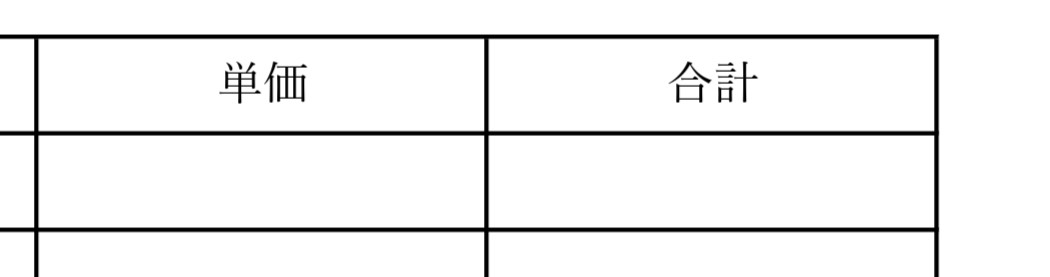
\includegraphics[width=15cm]{image/03-function/rect_original.jpg}
        }
        \caption{帳票画像にある矩形の記入欄}
        \label{fig:rect_original}
    \end{center}
\end{figure}

\begin{figure}[t]
    \begin{center}
        \fbox{
            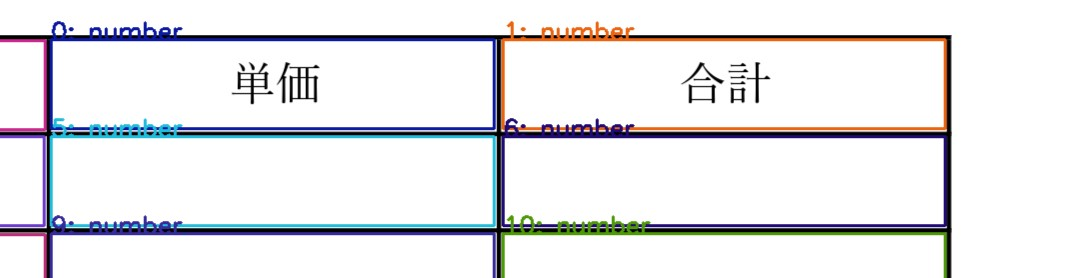
\includegraphics[width=15cm]{image/03-function/rects_with_label.jpg}
        }
        \caption{取得した矩形領域座標の描画}
        \label{fig:rect_drawing}
    \end{center}
\end{figure}

図\ref{fig:original}内にある帳票画像記入欄のうち、下線部の帳票画像記入欄を切り取った画像を、図\ref{fig:underline_original}に示す。
また、図\ref{fig:underline_original}の画像に対し、下線部の領域座標とラベルを取得し、描画した画像を、図\ref{fig:underline_drawing}に示す。
図\ref{fig:underline_drawing}の画像から、下線部の領域座標を参照して緑色で直線を描画し、同色で直線の左端点に番号と文字列を表示していることがわかる。
図\ref{fig:underline_drawing}の下線部に表示する番号は、JSONファイル内のunderlines\_data配列のidキーに対応する値と一致する。
同様に、番号の右に表示する文字列は、JSONファイル内のunderlines\_data配列のlabelキーに対応する値と一致する。
図\ref{fig:rect_drawing}の画像中にある、「御中」という文字の左にある下線部の左端点には、「0: number」と描画している。
これは、underlines\_data配列のidキーに0が、labelキーにstringがそれぞれ対応することを示す。

\begin{figure}[t]
    \begin{center}
        \fbox{
            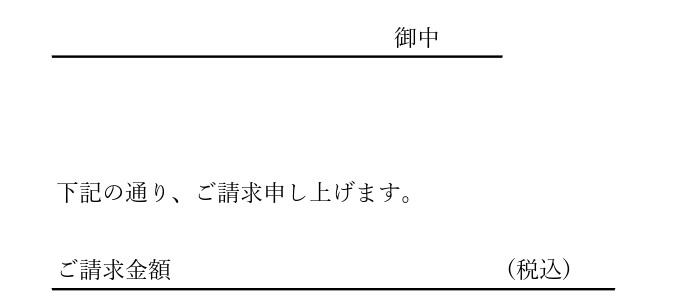
\includegraphics[width=15cm]{image/03-function/underline_original.jpg}
        }
        \caption{帳票画像にある下線部の記入欄}
        \label{fig:underline_original}
    \end{center}
\end{figure}

\begin{figure}[t]
    \begin{center}
        \fbox{
            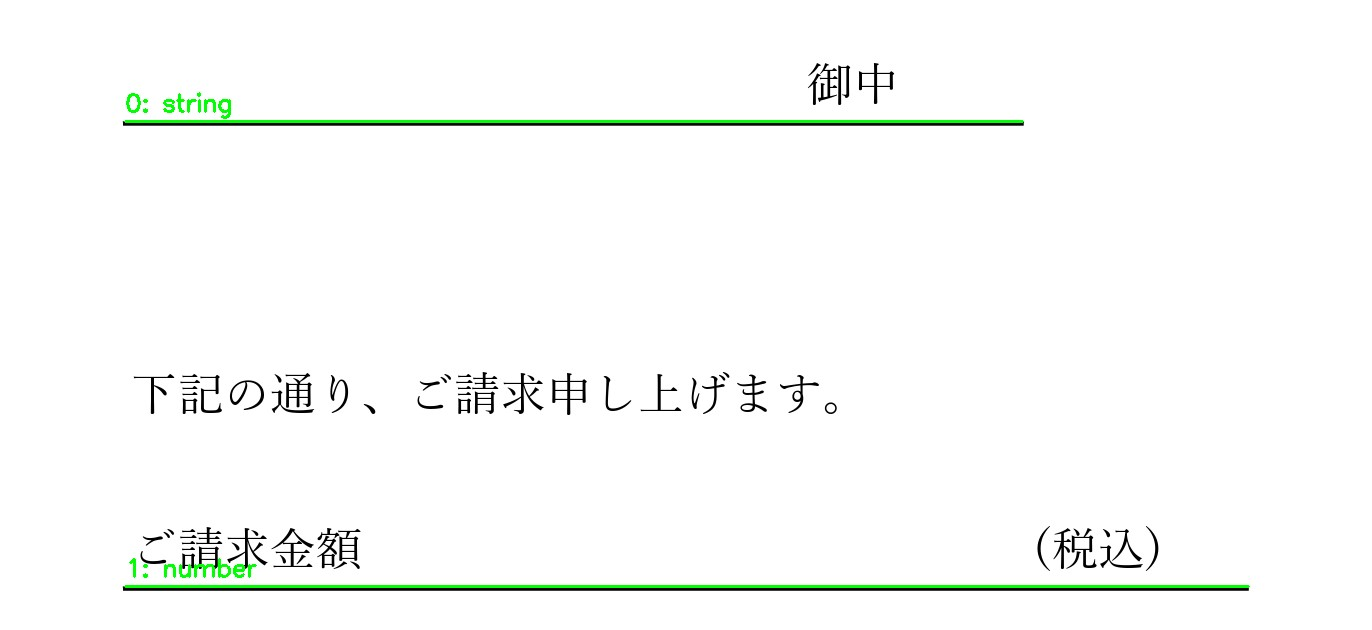
\includegraphics[width=15cm]{image/03-function/underlines_with_label.jpg}
        }
        \caption{取得した下線部領域座標の描画}
        \label{fig:underline_drawing}
    \end{center}
\end{figure}

図\ref{fig:rect_drawing}、図\ref{fig:underline_drawing}のように、入力である帳票画像に対して、領域座標を描画した画像を、本機能の出力の1つとする。

以上の2つの機能によって出力する、JSON形式のファイルと、PNG形式の画像2枚を、本提案手法の出力とする。

\chapter{本提案手法の実装}\label{cha:Implementation}
本提案手法は、領域座標取得部、文字情報取得部、ラベル付与部の3つの処理部で構成する。
本提案手法の構成を、図\ref{fig:structure}に示す。
以降、本章では3つの処理部について説明する。

\begin{figure}[t]
    \begin{center}
        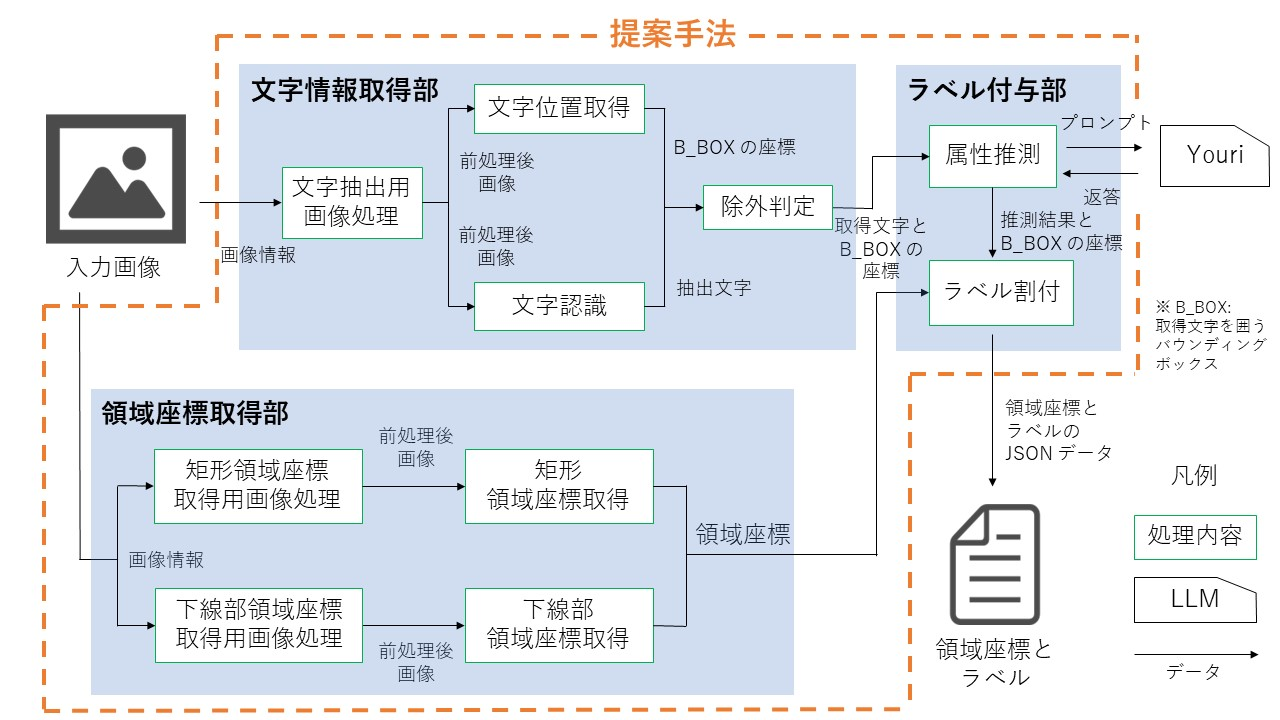
\includegraphics[width=15cm]{image/structure.jpg}
        \caption{本提案手法の構造}
        \label{fig:structure}
    \end{center}
\end{figure}


\section{領域座標取得部}\label{sec:area_coords_obtainment_part}
領域座標取得部は、帳票画像内記入欄を検出し、取得した座標を領域座標として出力する。
矩形の帳票画像記入欄については、各頂点のxy座標を、下線部の帳票画像記入欄については、両端点のxy座標を領域座標として取得する。
領域座標取得部の出力結果である領域座標は、ラベル付与部(\ref{subsec:label_link_processing}節で後述)で用いる。


\subsection{矩形領域座標取得処理}\label{subsec:rect_coords_obtainment_processing}
矩形領域座標取得処理は、矩形の記入欄を検出し、各頂点のxy座標を矩形領域座標として取得し、出力する処理である。
本処理の出力は、下線部領域座標取得処理(\ref{subsec:underline_coords_obtainment_processing})の一部で利用する。
矩形の取得にあたり、処理画像は白または黒でなければならないため、帳票画像に画像処理を施す必要がある。
以下に矩形領域座標の取得に必要な画像処理の順を示す。

\begin{enumerate}
    \item OpenCVのcvtColor関数を用いた、帳票画像のグレースケール化
    \item DeblurGANv2(\ref{sec:DeblurGANv2}節を参照)の適用によるブレ除去後のグレースケール化帳票画像の生成\\
        DeblurGANv2を適用することにより、スマートフォンで帳票画像を撮影する際に発生する画像内のブレを除去し、矩形の検出精度を高める。
    \item OpenCVのGaussianBlur関数(\ref{sec:OpenCV}節を参照)を用いた、ガウシアンフィルタによるノイズ除去\\
        本提案手法では、カーネルの縦幅と横幅を共に3、標準偏差を0とする。
    \item OpenCVのthreshold関数(\ref{sec:OpenCV}節を参照)を用いた、大津の二値化による二値画像への変換\\
        本提案手法では、閾値処理を大津の二値化としたTHRESH\_TOZERO\_INVによる二値化手法とする(\ref{sec:OpenCV}節を参照)。
        白黒を反転して二値化することにより、複数の矩形が隣接する場合に、それらを外接する最小の外接矩形を不要に検出してしまうことを防ぐ。
    \item OpenCVのgetStructuringElement関数(\ref{sec:OpenCV}節を参照)を用いた、カーネルの作成\\
        本提案手法では、5行5列の矩形カーネルを作成する。
\end{enumerate}

スマートフォンのカメラで撮影する際にブレが生じた帳票画像を図\ref{fig:before_deblur}に示す。
図\ref{fig:before_deblur}に対して、DeblurGANv2を適用することによってブレを除去した画像を図\ref{fig:after_deblur}に示す。
図\ref{fig:before_deblur}と図\ref{fig:after_deblur}より、DeblurGANv2によるブレ除去によって、図\ref{fig:before_deblur}でブレている矩形の線が図\ref{fig:after_deblur}ではっきりとなっていることがわかる。

\begin{figure}[t]
    \centering
    \begin{minipage}[t]{0.45\linewidth}
      \centering
      \fbox{
        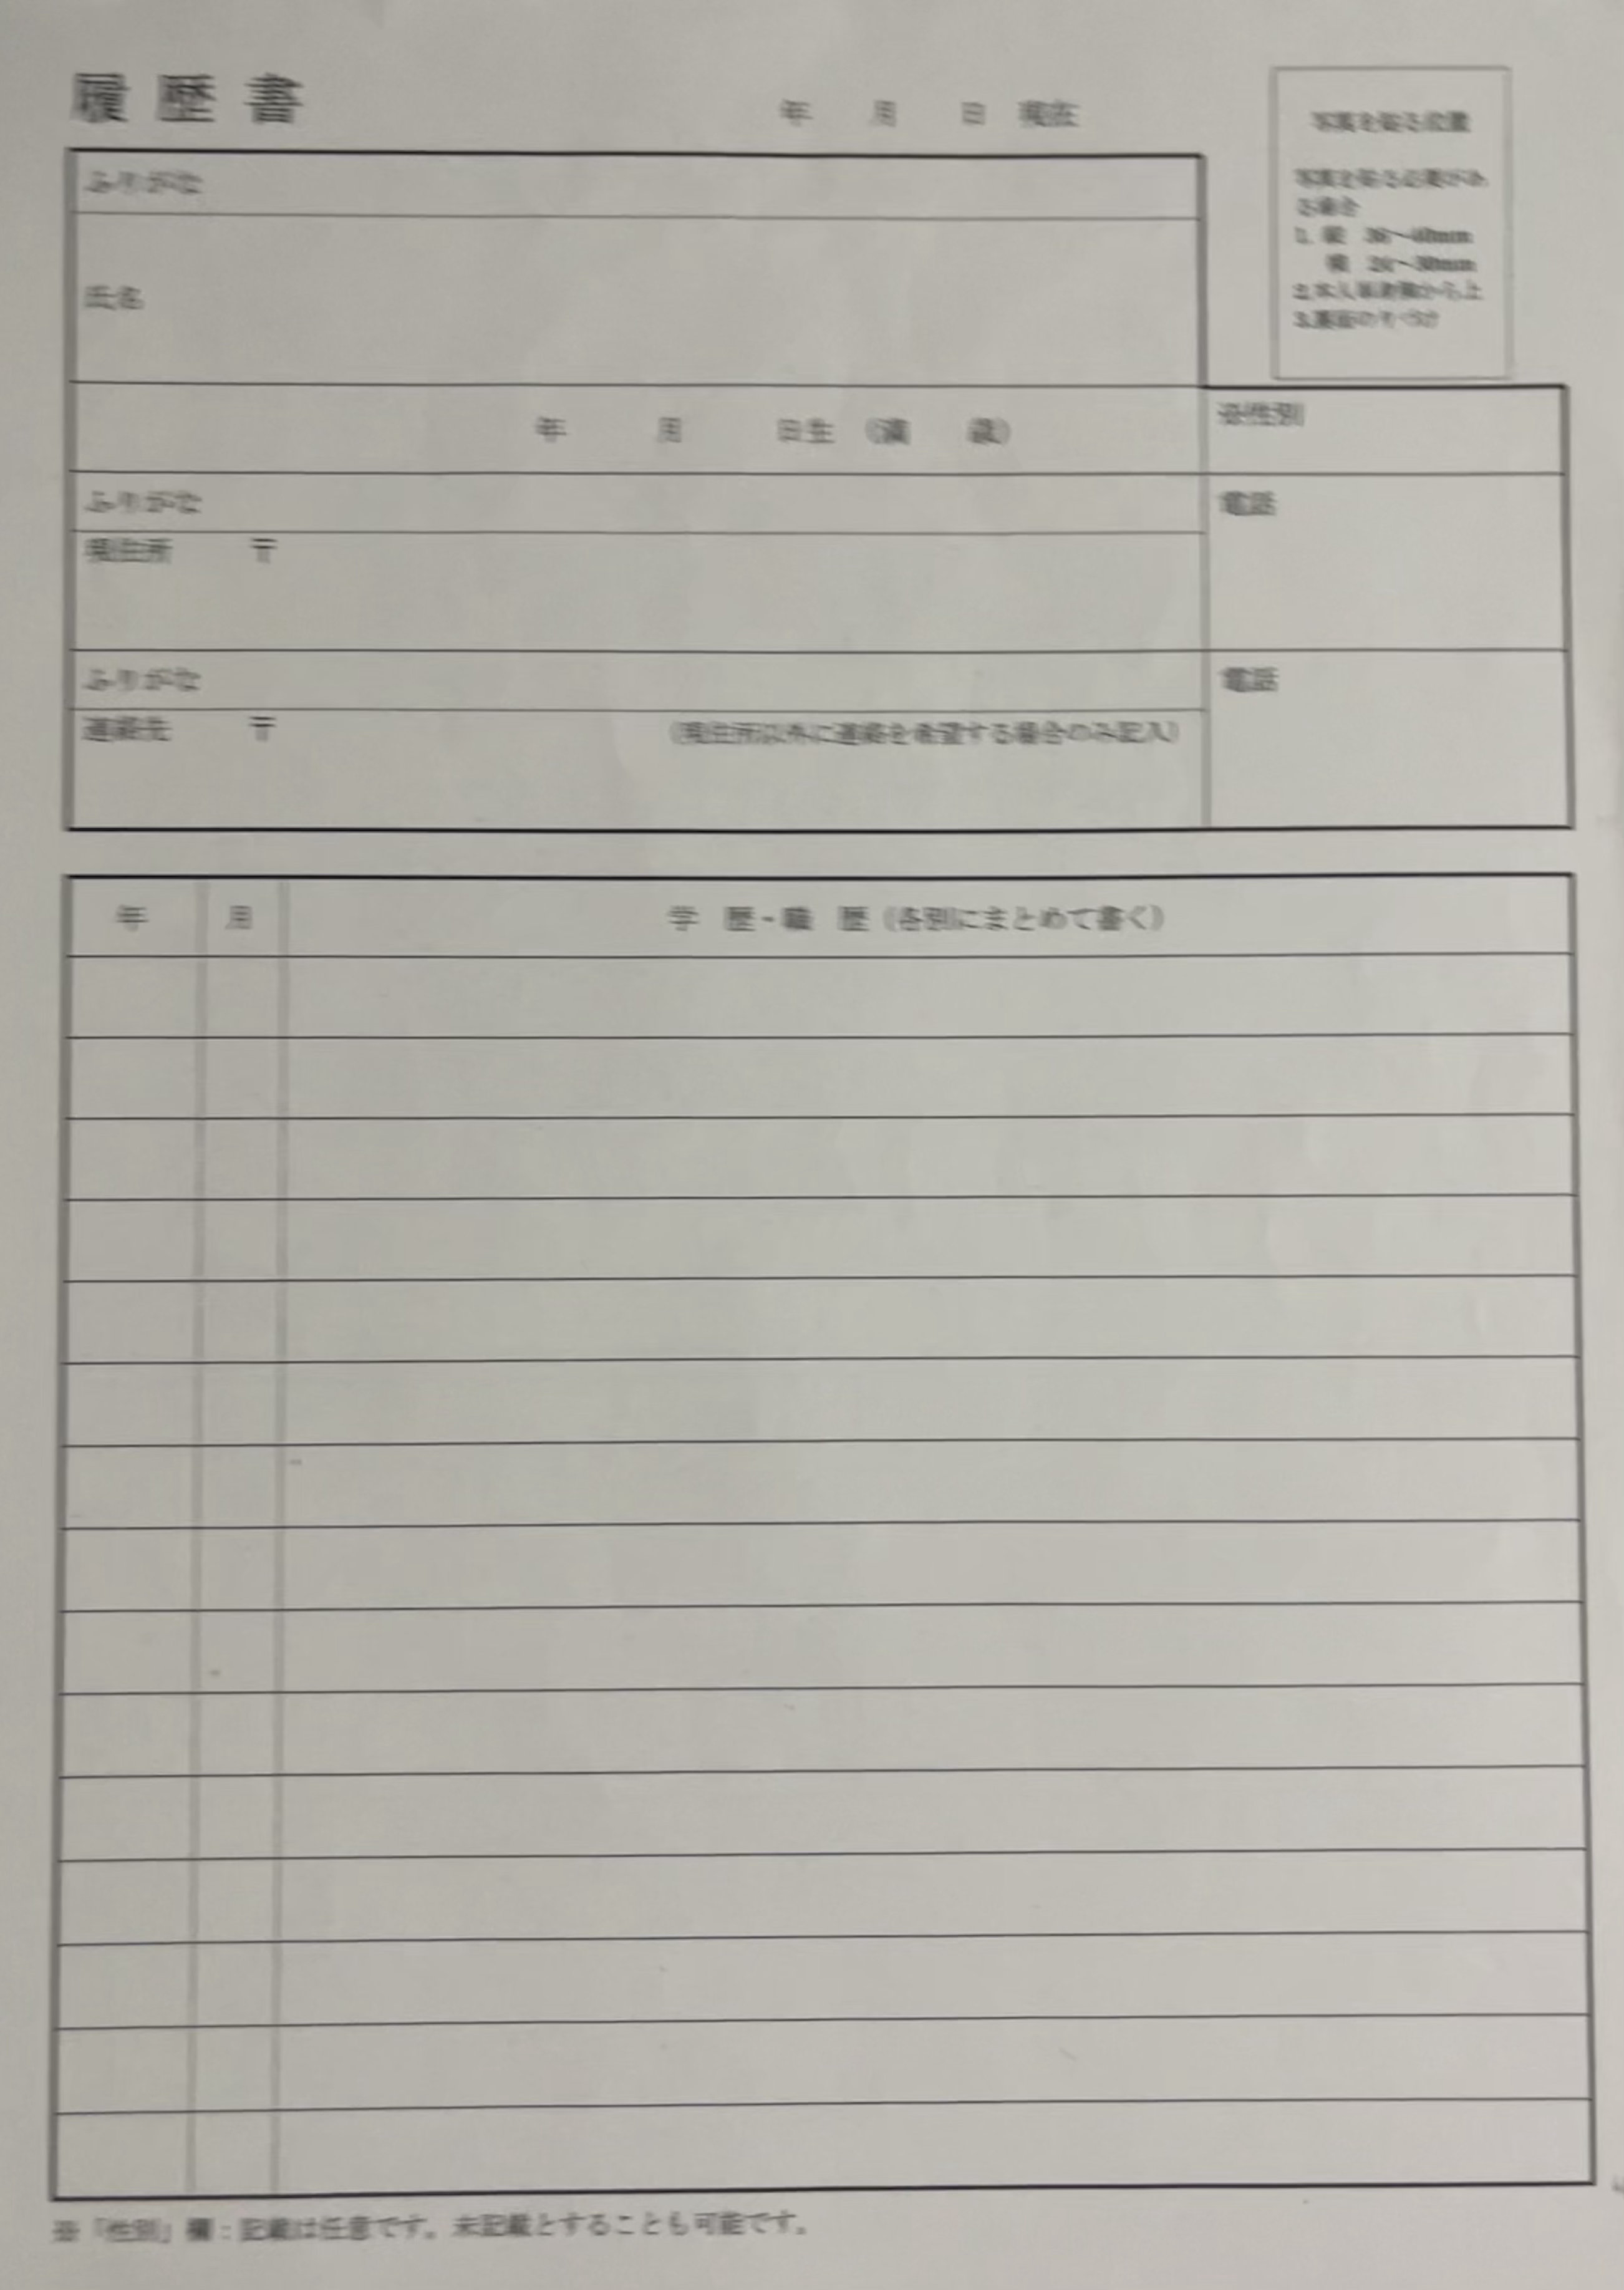
\includegraphics[keepaspectratio, width=7cm]{image/04-implementation/before_deblur.png}
      }
      \caption{撮影するにあたってブレが生じた帳票画像}
      \label{fig:before_deblur}
    \end{minipage}
    \begin{minipage}[t]{0.45\linewidth}
      \centering
      \fbox{
        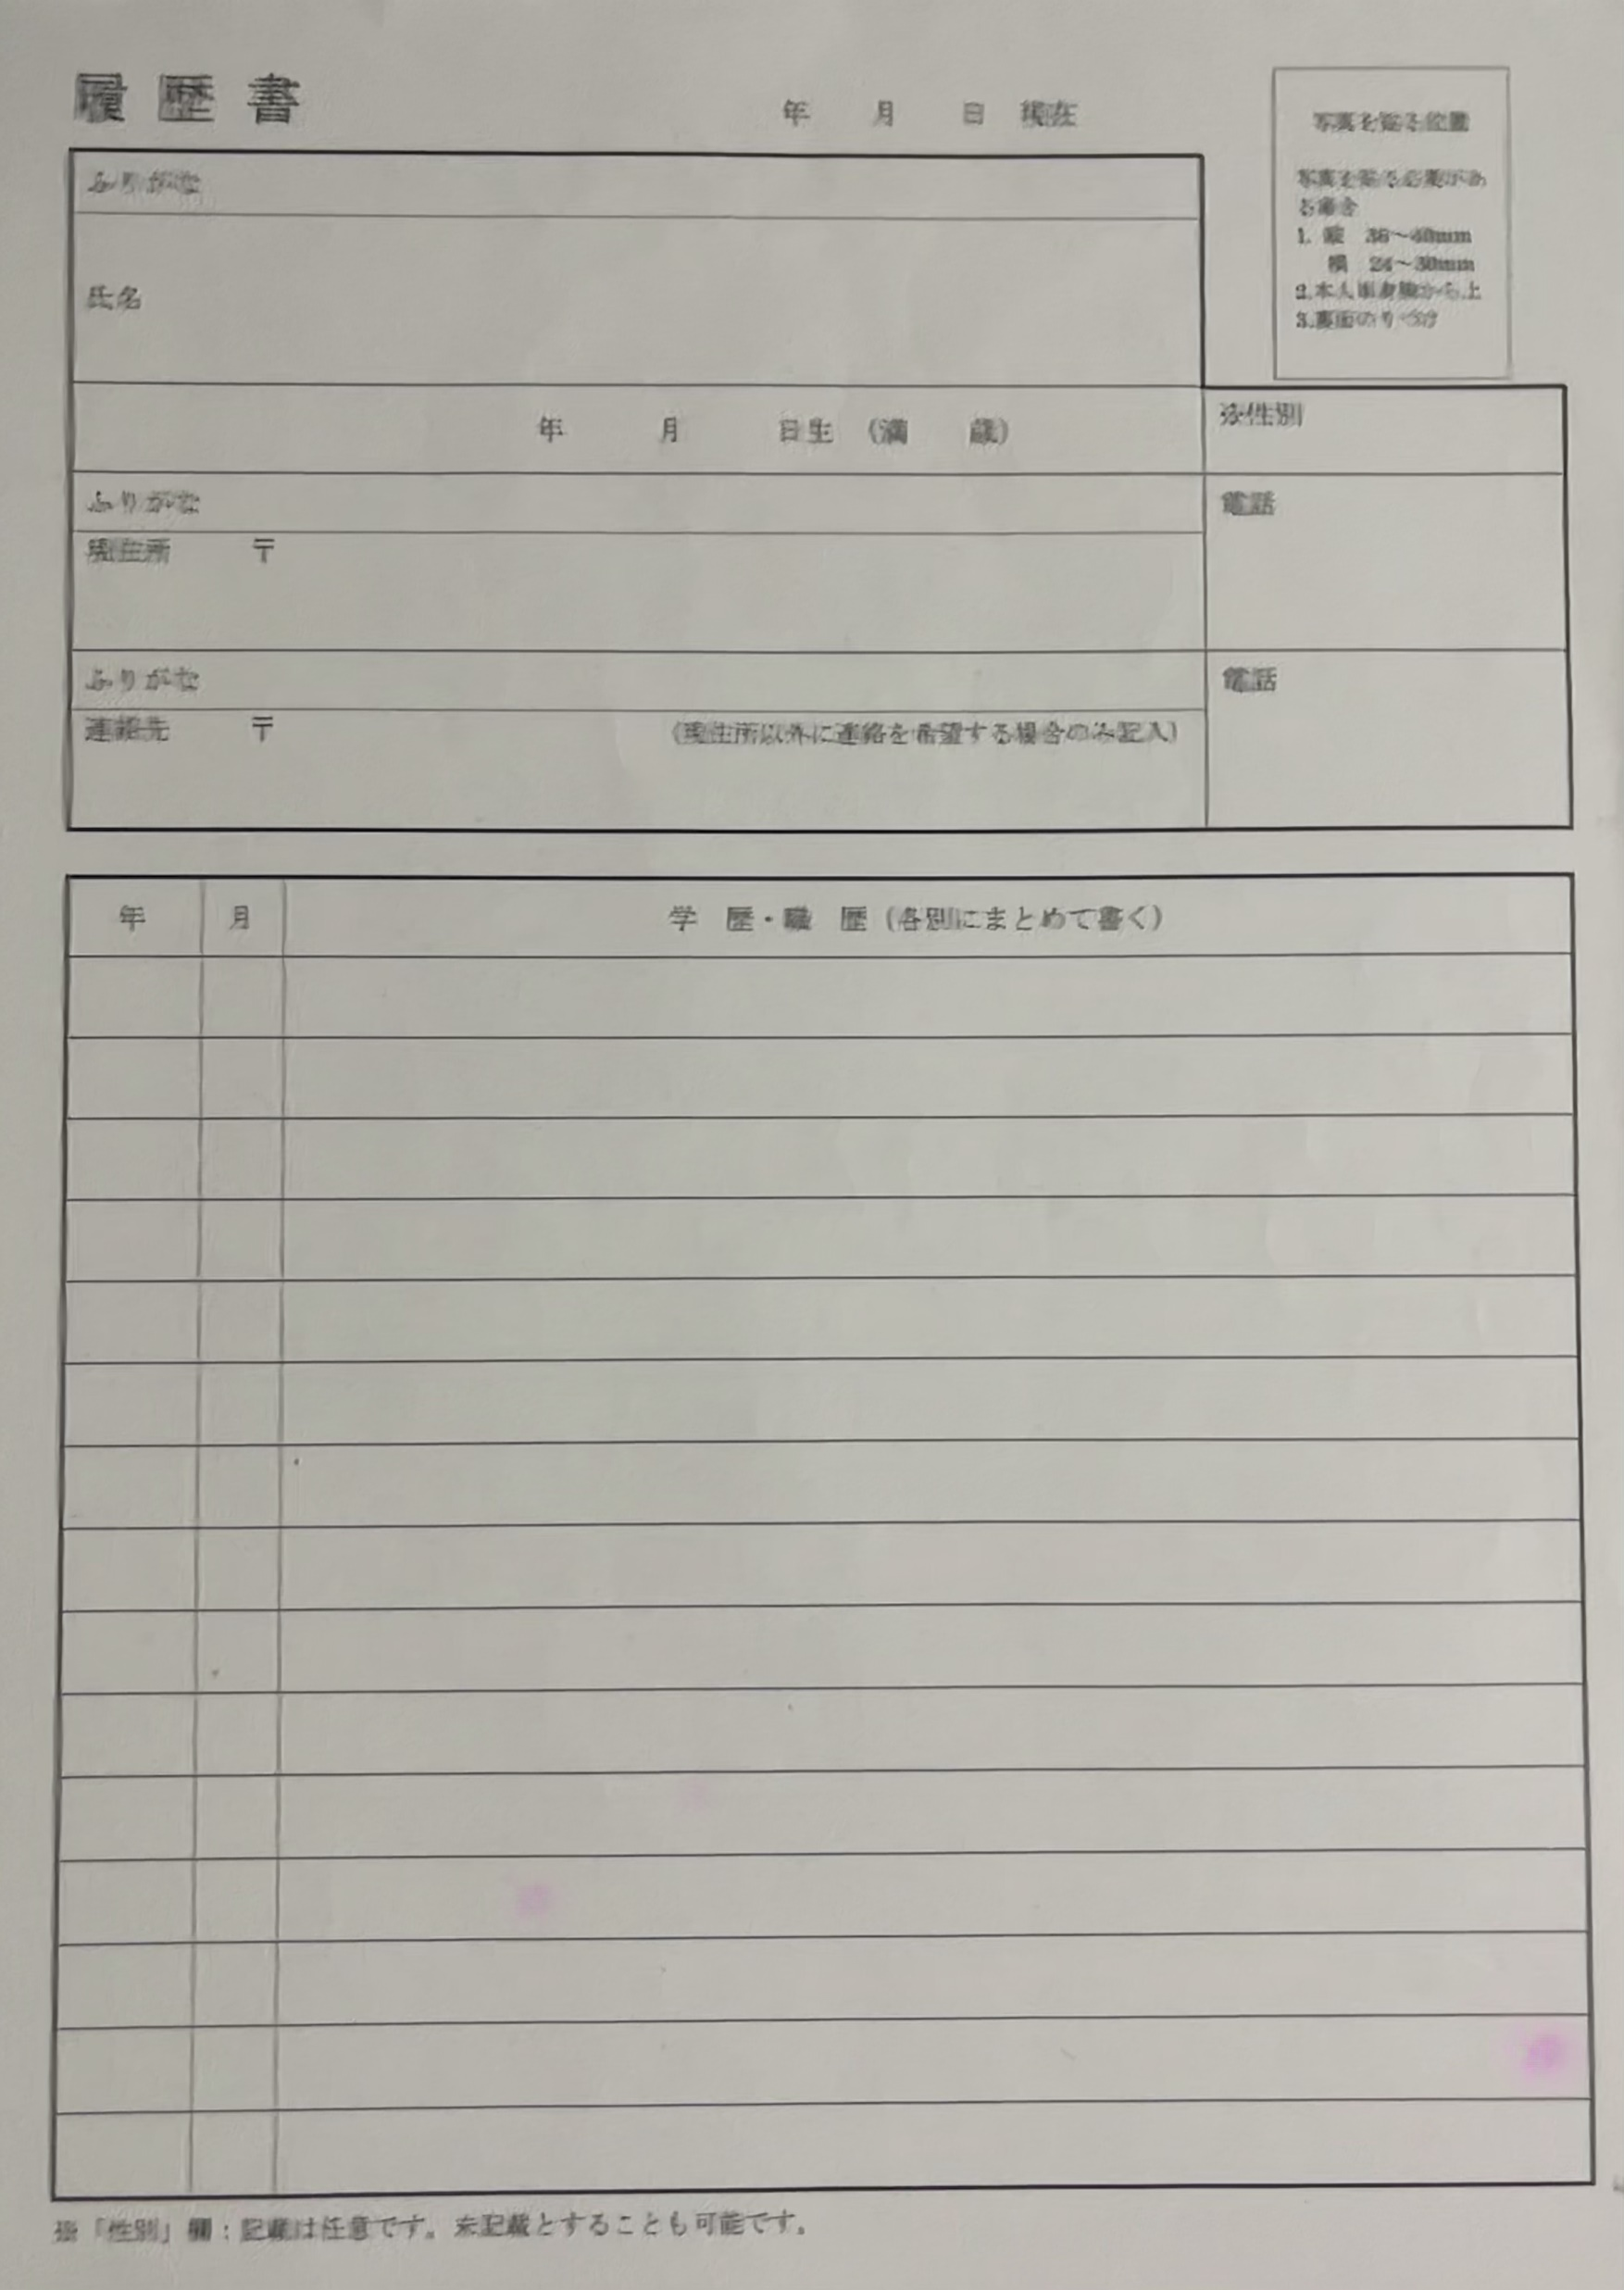
\includegraphics[keepaspectratio, width=7cm]{image/04-implementation/after_deblur.jpeg}
      }
      \caption{発生したブレを除去した帳票画像}
      \label{fig:after_deblur}
    \end{minipage}
\end{figure}

画像処理後、OpenCVのfindContours関数(\ref{sec:OpenCV}節を参照)による輪郭検出を用いて矩形の帳票画像記入欄を検出し、矩形領域座標を取得する。
なお、以下の条件のいずれかに該当する矩形については、記入欄として不適切であり誤検知の場合があるとして、出力の対象外とする。

\begin{itemize}
    \item 面積が3000ピクセル以下である場合
    \item ある辺の長さが10ピクセル以下である場合
\end{itemize}

DeblurGANv2によるブレ除去を行っていない画像を示す図\ref{fig:before_deblur}に対して、矩形領域座標取得処理の出力結果を描画した画像を図\ref{fig:before_deblur_area}に示す。
DeblurGANv2によるブレ除去を行った画像を示す図\ref{fig:after_deblur}に対し、DeblurGANv2を適用することによってブレを除去した画像を入力として、矩形領域座標取得処理の出力結果を描画した画像を図\ref{fig:after_deblur_area}に示す。
図\ref{fig:before_deblur_area}と図\ref{fig:after_deblur_area}より、DeblurGANv2によるブレ除去によって、矩形領域の検出精度が向上していることがわかる。

\begin{figure}[t]
    \centering
    \begin{minipage}[t]{0.45\linewidth}
      \centering
      \fbox{
        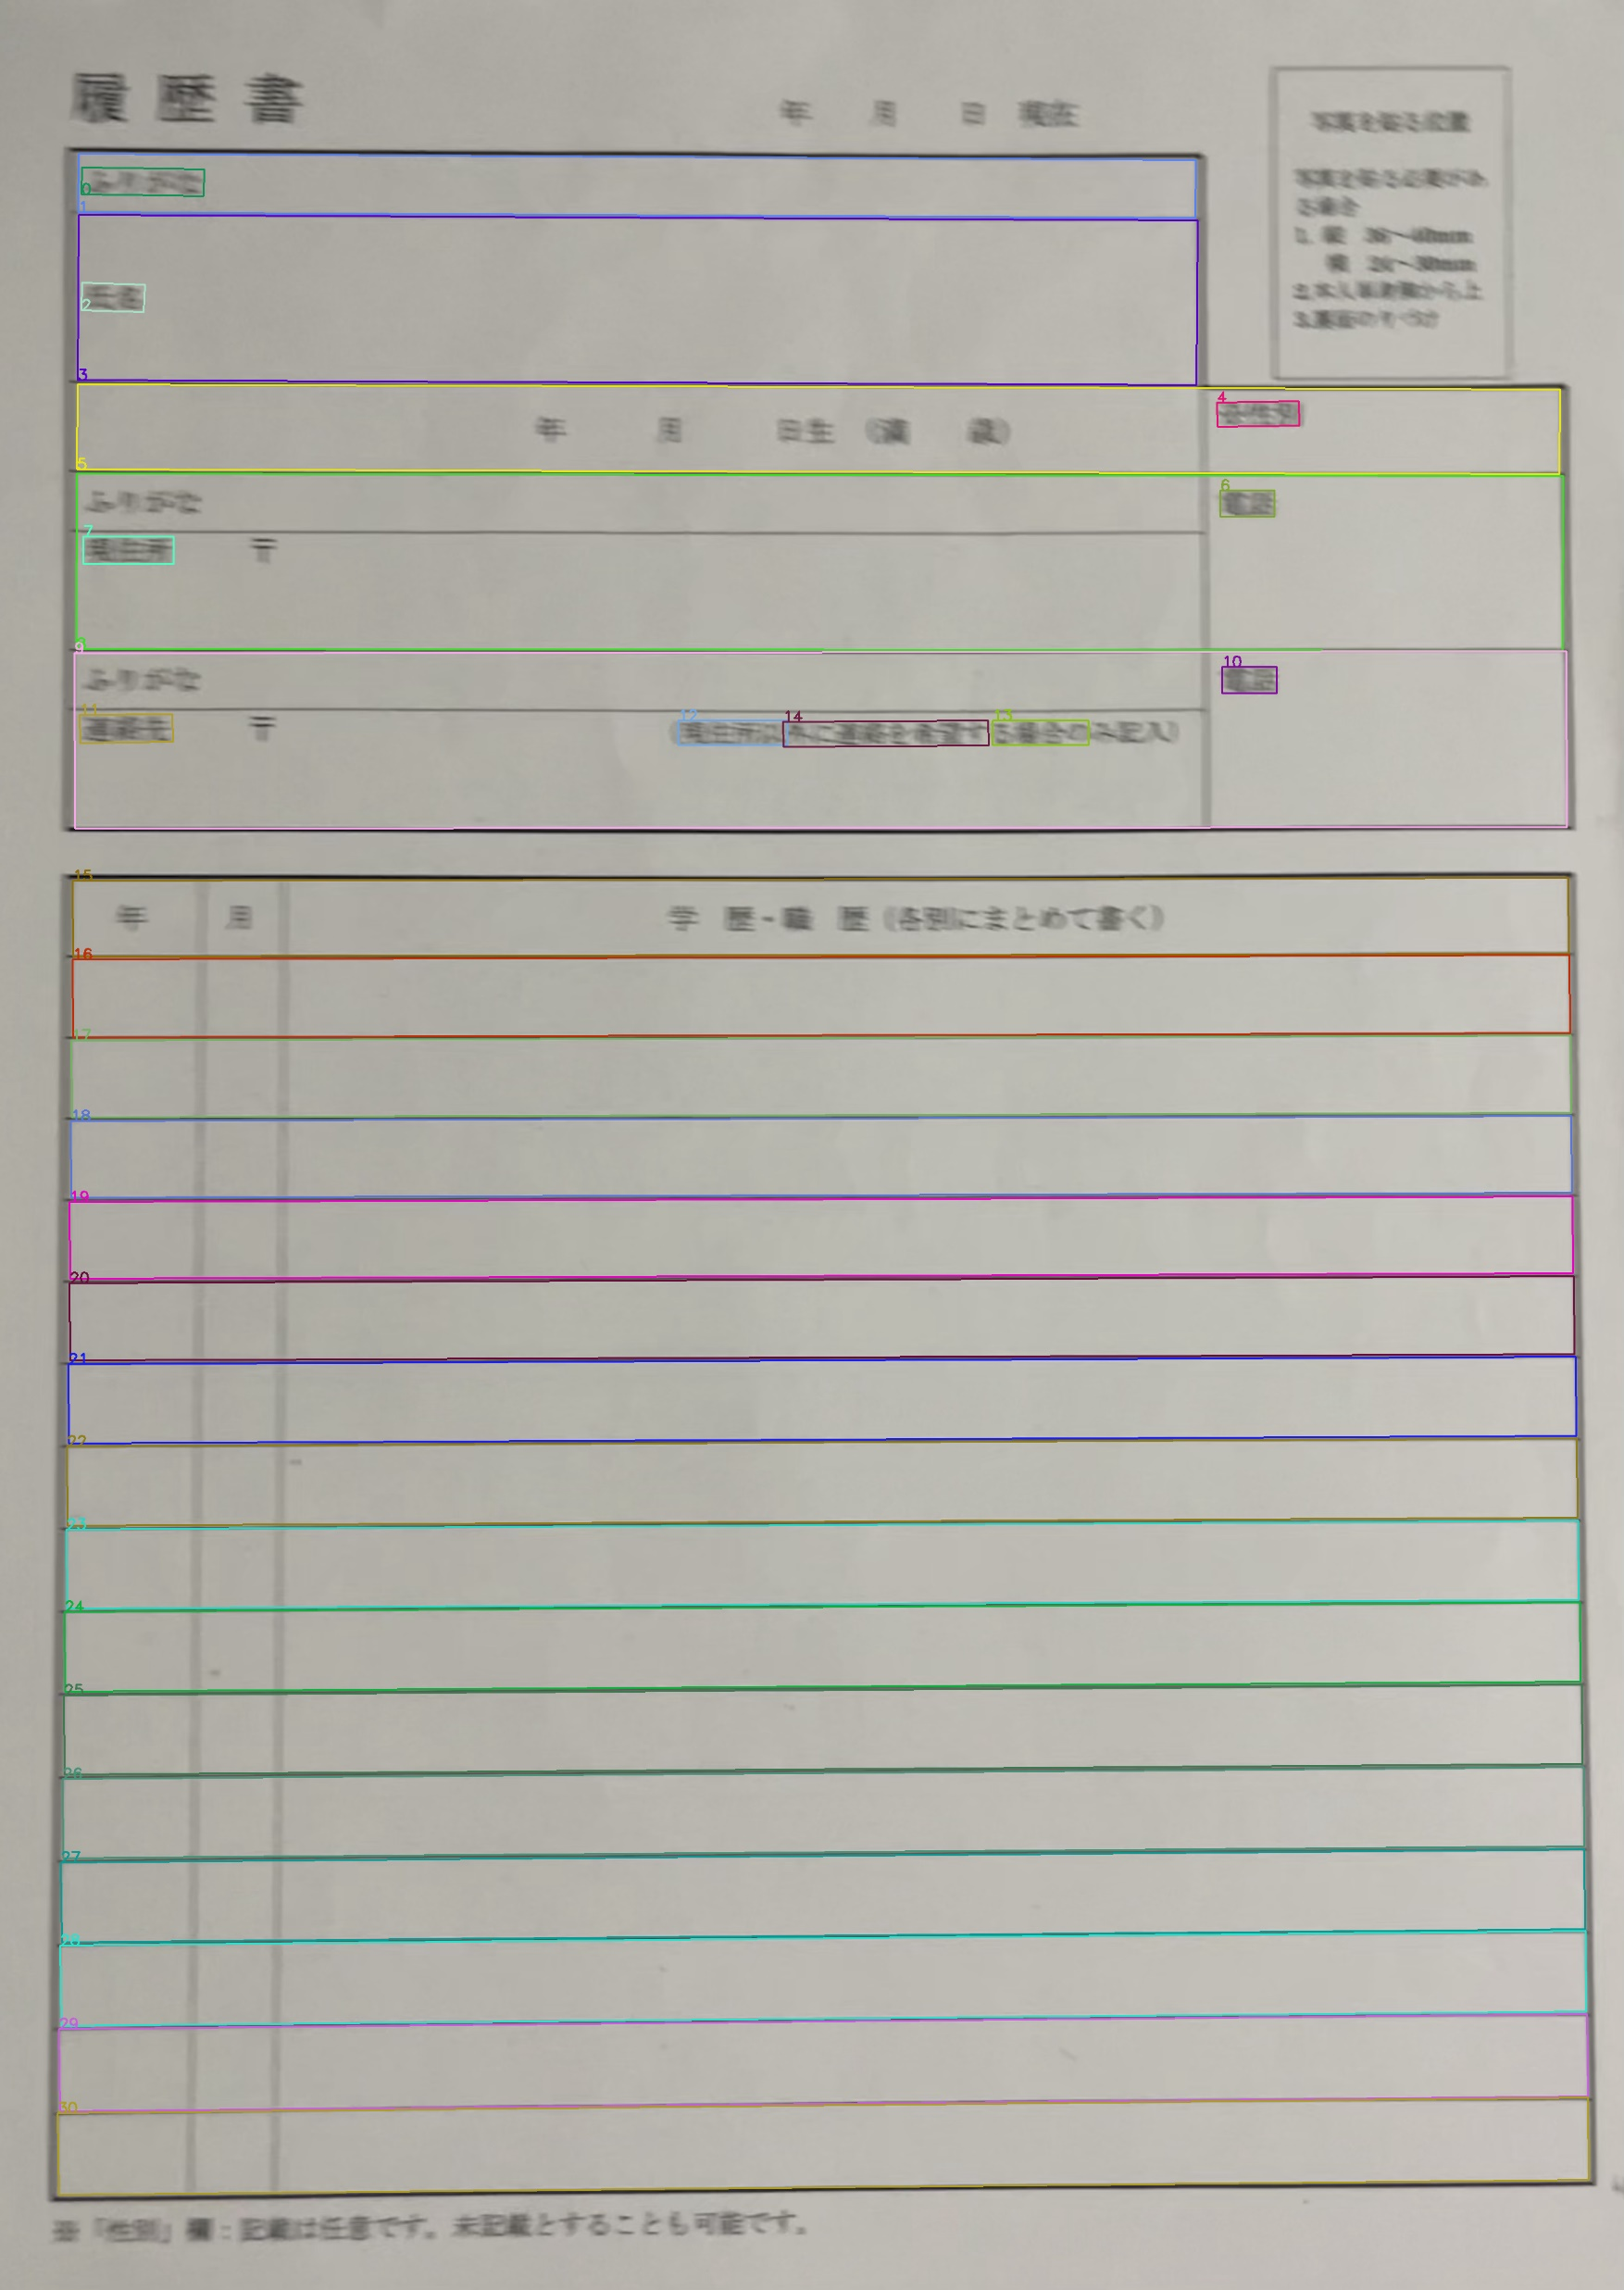
\includegraphics[keepaspectratio, width=7cm]{image/04-implementation/before_deblur_area.jpeg}
      }
      \caption{DeblurGANv2を適用していないブレのある帳票画像の領域座標取得処理の出力}
      \label{fig:before_deblur_area}
    \end{minipage}
    \begin{minipage}[t]{0.45\linewidth}
      \centering
      \fbox{
        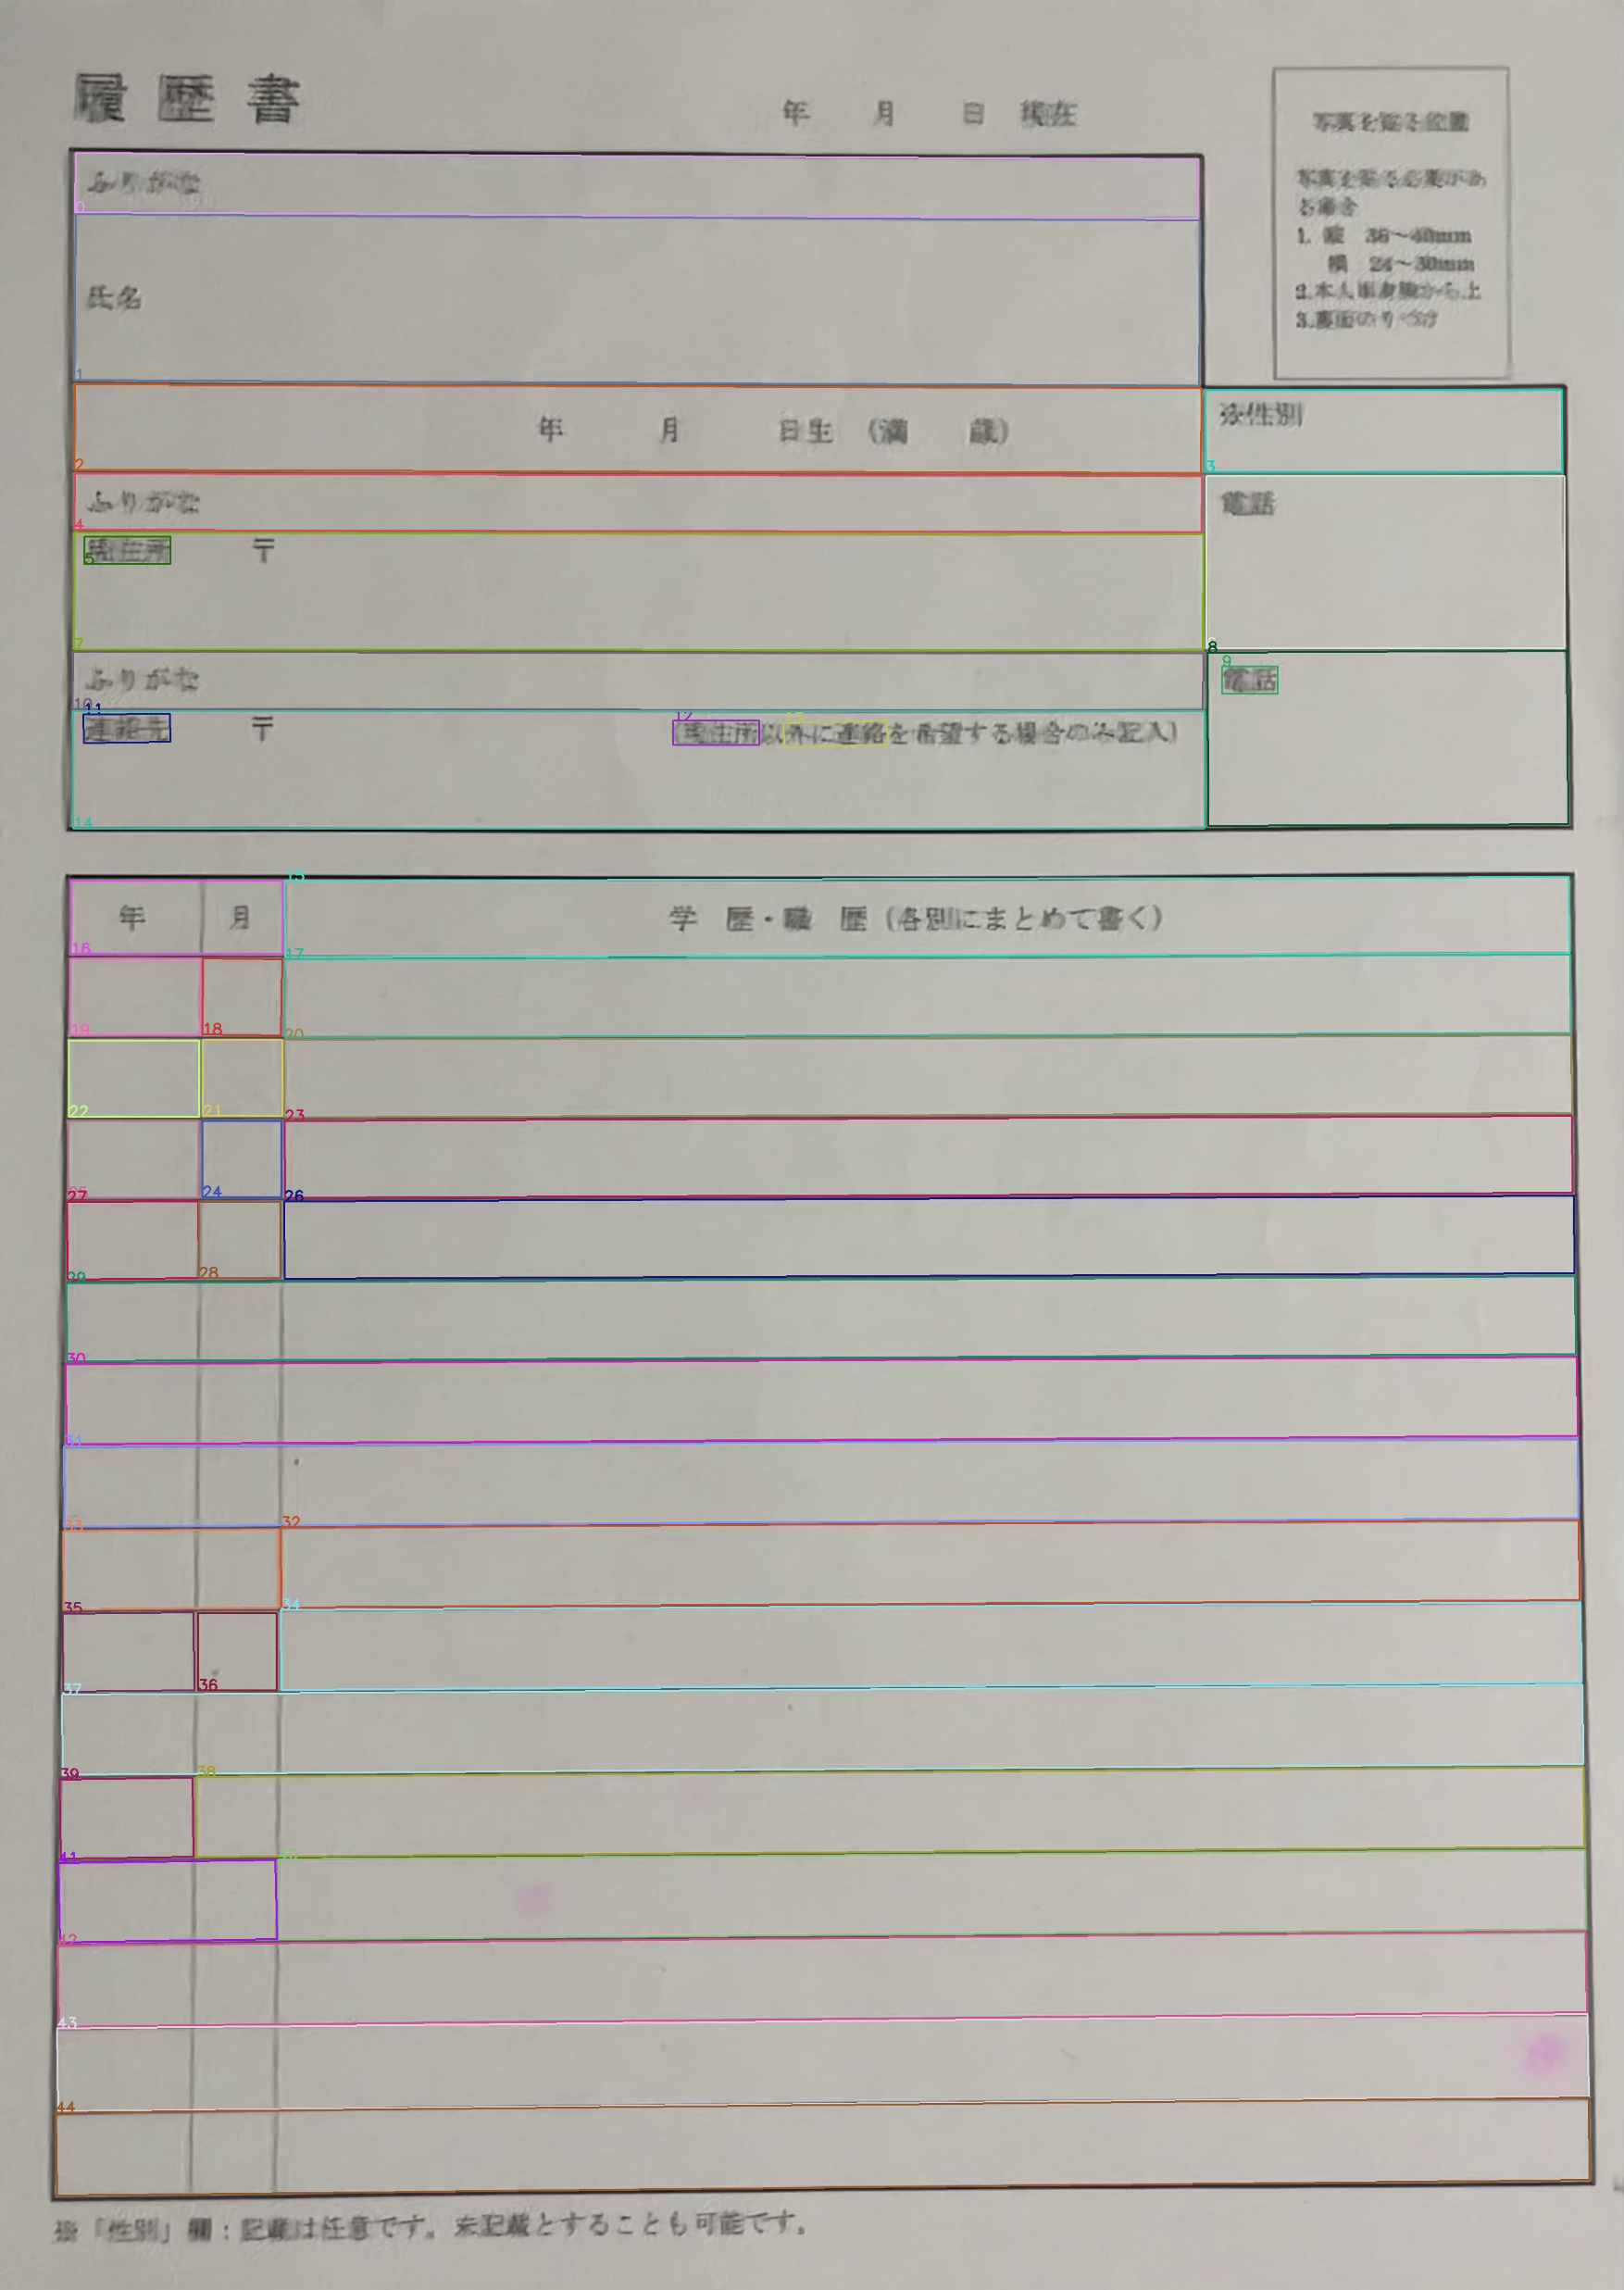
\includegraphics[keepaspectratio, width=7cm]{image/04-implementation/after_deblur_area.jpeg}
      }
      \caption{DeblurGANv2適用後のブレを除去した帳票画像の領域座標取得処理の出力}
      \label{fig:after_deblur_area}
    \end{minipage}
\end{figure}




\subsection{下線部領域座標取得処理}\label{subsec:underline_coords_obtainment_processing}
下線部領域座標取得処理は、下線部の記入欄を検出し、両端点のxy座標を下線部領域座標として取得し、出力する処理である。
下線部の取得にあたり、処理画像は白または黒でなければならないため、帳票画像に画像処理を施す必要がある。
以下に下線部領域座標の取得に必要な画像処理の順を示す。
なお、本処理における画像処理の一部は、矩形領域座標取得処理(\ref{subsec:rect_coords_obtainment_processing}節)と同様の画像処理を施す。

\begin{enumerate}
    \item OpenCVのcvtColor関数を用いた、帳票画像のグレースケール化\\
        \ref{subsec:rect_coords_obtainment_processing}節と同様の処理
    \item DeblurGANv2の適用によるブレ除去後のグレースケール化帳票画像の生成\\
        \ref{subsec:rect_coords_obtainment_processing}節と同様の処理
    \item OpenCVのthreshold関数を用いた、大津の二値化による二値画像への変換\\
        本提案手法では、閾値処理を大津の二値化としたTHRESH\_BINARYによる二値化手法とする。
    \item OpenCVのthreshold関数(\ref{sec:OpenCV}節を参照)を用いた、Canny法によるエッジ検出\\
        本提案手法では、閾値処理における上限と下限の閾値を、以下のように決定する。
        \begin{enumerate}
            \item 構成画素の画素値の中央値を取得する。
            \item 中央値の定数倍(本研究では定数を0.33とする)を、取得した中央値から加減算する。
            \item 加算した値を上限の閾値、減算した値を下限の閾値として設定する。
        \end{enumerate}
\end{enumerate}

画像処理後、OpenCVのHoughLinesP関数(\ref{sec:OpenCV}節を参照)によるハフ変換を用いて下線の帳票画像記入欄を検出し、下線部領域座標を取得する。
なお、以下の条件のいずれかに該当する直線については、記入欄として不適切であり誤検出の場合があるとして、出力の対象外とする。
条件の1つに矩形領域座標取得処理(\ref{subsec:rect_coords_obtainment_processing}節)の出力を利用する。

\begin{itemize}
    \item 直線の長さが10ピクセル未満である場合
        Canny法で適用するガウシアンフィルタで除去できていないノイズによって誤検出したエッジを下線と捉えることを防ぐ。
    \item 水平を基準として傾きが3ピクセル以上である場合
        横書きの帳票において、下線部の直線は水平であるため、垂直な直線を下線と捉えることを防ぐ。
    \item 直線が矩形領域の辺の一部から上下20ピクセル以内に存在する場合\\
        矩形領域座標取得処理の出力を利用する。矩形領域の辺の一部を下線と捉えることを防ぐ。
\end{itemize}

エッジ検出を施すことにより、直線の検出精度が向上するが、直線の上下に2本の直線を検出してしまう場合がある。
これに対しては、検出した直線の中点を全て計算し、ある直線における中点のy座標について、上下10ピクセル以内に別の直線の中点が存在する場合は、二直線の両端点のxy座標をそれぞれ平均して一本の直線に統一することによって不具合を解消する。

\section{文字情報取得部}\label{sec:OCR_part}
文字情報取得部では、光学文字認識(\ref{sec:Optical-Charactor-Recognition}節を参照)によって、帳票画像内の文字についての情報を取得する。
本提案手法では、光学文字認識ソフトTesseract-OCRを用いて、文字と、文字を囲うバウンディングボックスの各頂点のxy座標を文字位置として取得する。
文字情報取得部の出力結果は、ラベル付与部(\ref{subsec:label_link_processing}節で後述)で用いる。

\subsection{文字認識処理}\label{subsec:char_recognition_processing}
文字認識処理は、認識した文字を取得文字として取得する処理である。
文字の取得にあたり、文字の認識精度を高めるため、以下の順で帳票画像に画像処理を施す。

\begin{enumerate}
    \item DeblurGANv2の適用によるブレ除去後のグレースケール化帳票画像の生成\\
        \ref{subsec:rect_coords_obtainment_processing}節と同様の処理
    \item OpenCVのcvtColor関数を用いた、帳票画像のグレースケール化\\
        \ref{subsec:rect_coords_obtainment_processing}節と同様の処理
    \item OpenCVのthreshold関数を用いた、大津の二値化による二値画像への変換\\
        本提案手法では、閾値処理を大津の二値化としたTHRESH\_BINARYによる二値化手法とする。
\end{enumerate}

画像処理後、Tesseract-OCRによる文字認識を行う。文字認識処理と同時に、文字認識処理(\ref{subsec:char_recognition_processing}節)を行う。


\subsection{文字位置取得処理}\label{subsec:char_position_obtainment_processing}
文字位置取得処理は、認識した文字を囲うバウンディングボックスの各頂点のxy座標を文字位置として取得する処理である。
本処理は文字認識処理(\ref{subsec:char_recognition_processing}節)と同時に行い、文字位置を取得する。

文字位置取得後、バウンディングボックスの左上の頂点座標について、y座標の値が小さい順に文字認識処理(\ref{subsec:char_recognition_processing}節)で取得した文字と組とし、番号を割り振る。y座標が同じ場合は、さらにx座標が小さい順にソートする。
しかし、人間の目視で複数の文字列が同じ行に存在すると認識するとき、左右の順番がバラバラとなる場合がある。
これは、Tesseract-OCRが文字を認識する順番を、y座標についてピクセル単位で降順にソートするため、人間の目視で認識する順番とソート後の順番に違いが生じるためである。
ラベル付与部(\ref{subsec:label_link_processing}節で後述)で文字位置を扱う際に、ソート結果が人間の認識と異なる場合、ラベルの更新順が変化してしまうため、意図しないラベルを領域座標に割り付ける不具合が発生する場合がある。
この不具合の発生を防ぐため、ソートで比較する値は、y座標を10分の1にした値(小数点以下切り捨て)を用いてソートを行う。

ある帳票画像に対して文字位置取得処理を施し、同一行における取得文字の左右の順番をバラバラに認識した場合のバウンディングボックスの画像を図\ref{fig:before_sorted_string}に示す。
図\ref{fig:before_sorted_string}内の12番から15番について、左から14番、15番、13番、12番となっている。
これに対し、y座標を10分の1にした値で比較することにより、左右の順番を左から右へ番号が大きくなるようソートした場合のバウンディングボックスの画像を図\ref{fig:after_sorted_string}に示す。
ソート後は、図\ref{fig:after_sorted_string}内における12番から15番は、左から12番、13番、14番、15番となっており、左右の順番を入れ替えることに成功していることがわかる。

\begin{figure}[t]
    \begin{center}
        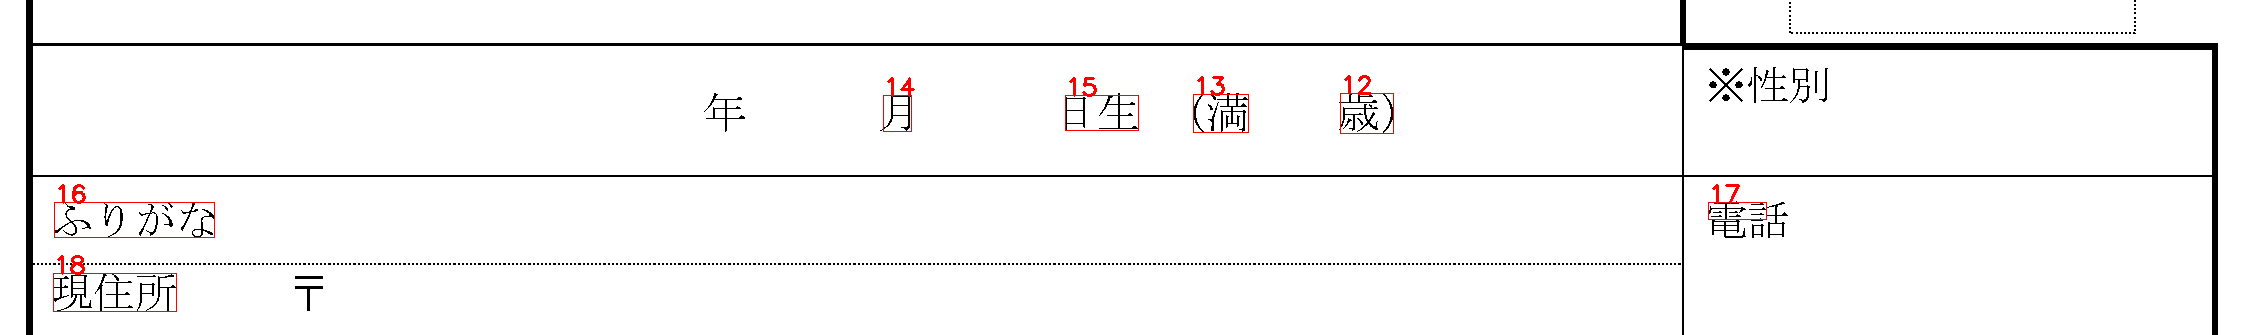
\includegraphics[width=15cm]{image/04-implementation/before_sorted_string.png}
        \caption{左右の順番をバラバラに認識した文字位置取得処理の出力}
        \label{fig:before_sorted_string}
    \end{center}
\end{figure}

\begin{figure}[t]
    \begin{center}
        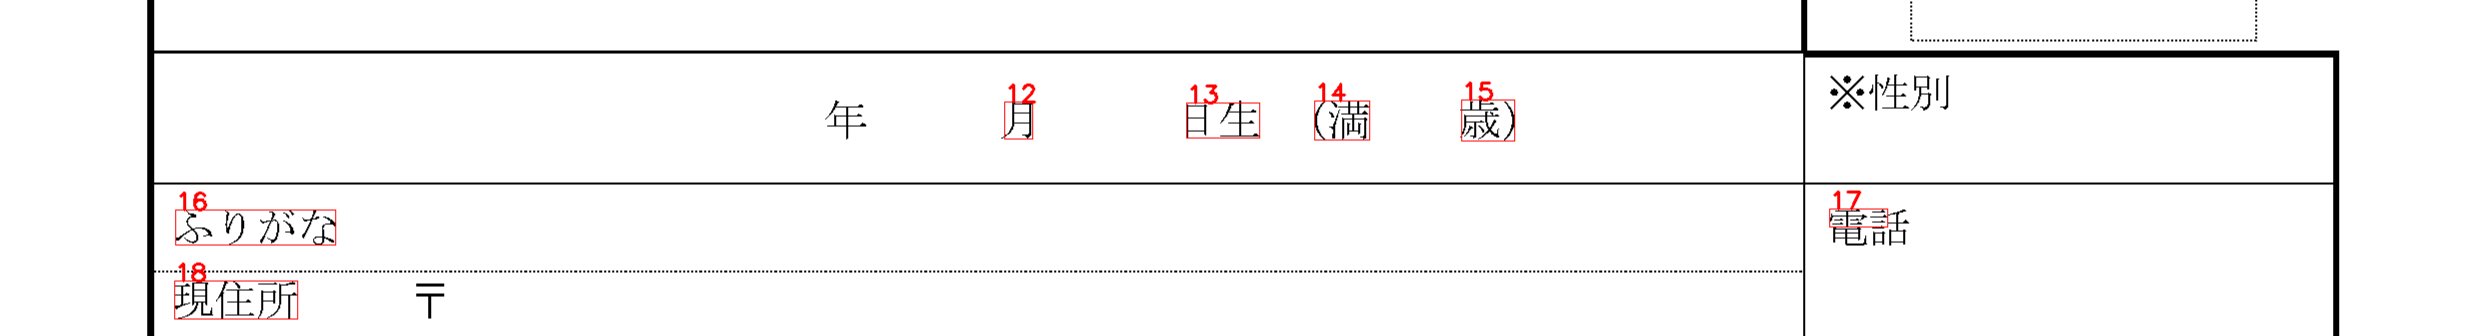
\includegraphics[width=15cm]{image/04-implementation/after_sorted_string.png}
        \caption{同行の番号を左から右へ昇順となるようソートした文字位置取得処理の出力}
        \label{fig:after_sorted_string}
    \end{center}
\end{figure}


\subsection{除外判定処理}\label{subsec:exclusion_judgement_processing}
除外判定処理は、Fugashi(\ref{sec:Fugashi}節を参照)による形態素解析を行い、属性判定処理(\ref{subsec:att_prediction_processing}節で後述)に不要である取得文字について、出力から除外する処理である。
形態素の品詞を解析し、取得文字の構成形態素数のうち、特定の品詞である形態素数の割合が半分以上である場合は、属性判定において意味がない取得文字であるとして、該当の取得文字と文字位置を文字情報取得部の出力から除外する。
文字を認識する際に、紙面と背景の境界や、矩形や直線を文字として誤認識する場合がある。
不要な文字の属性推測を防ぐことにより、処理時間を短縮することが可能である。

除外対象である形態素の品詞を、UniDic品詞体系(左からカンマ区切りで、大分類、中分類、小分類、細分類)をもとに以下に示す。
なお、除外対象とする品詞は経験から決定している。

\begin{itemize}
    \item 補助記号,一般,*,*
    \item 感動詞,フィラー,*,*
\end{itemize}

ある帳票画像に対して、認識した文字のバウンディングボックスを描画した画像の一部を図\ref{fig:before_exclusion_bbox}に示す。
図\ref{fig:before_exclusion_bbox}の文字認識の結果の画像を図\ref{fig:before_exclusion_string}に示す。
図\ref{fig:before_exclusion_bbox}、図\ref{fig:before_exclusion_string}内の58番および60番は、帳票画像内の矩形を誤って文字として認識しており、取得文字は属性判定において意味がない文字である。
図\ref{fig:before_exclusion_string}に対して除外判定処理を適用し、属性判定に不要な取得文字を除外した出力を図\ref{fig:after_exclusion_string}に示す。
図\ref{fig:after_exclusion_string}より、属性判定に不要な取得文字の除外に成功していることがわかる。

\begin{figure}[t]
    \begin{center}
        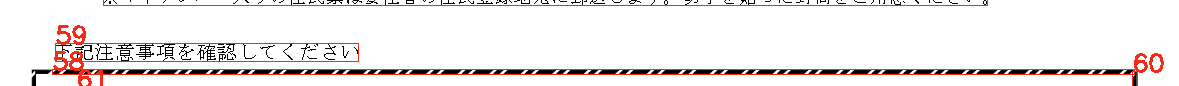
\includegraphics[width=15cm]{image/04-implementation/before_exclusion_bbox.png}
        \caption{属性判定に不要な文字を含む文字認識}
        \label{fig:before_exclusion_bbox}
    \end{center}
\end{figure}

\begin{figure}[t]
    \begin{center}
        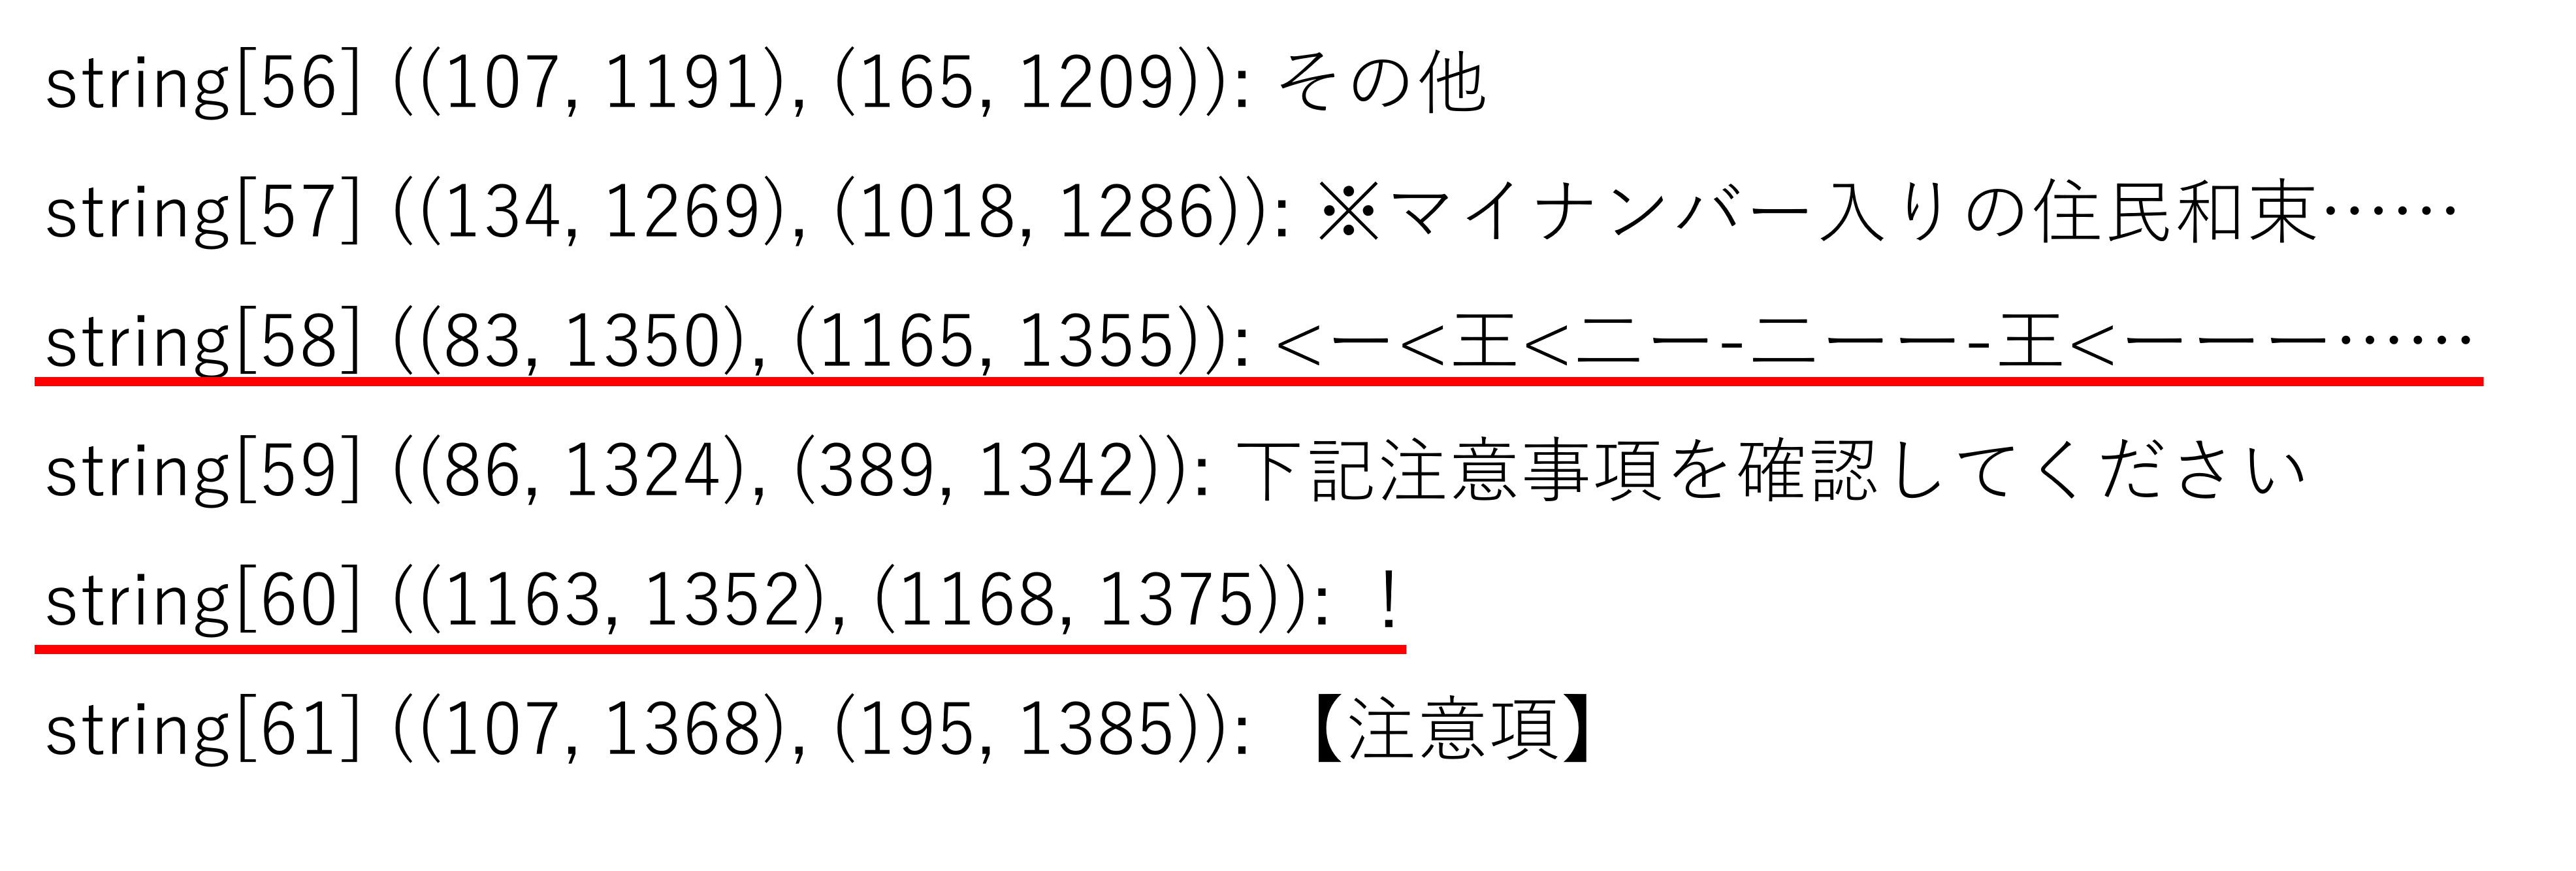
\includegraphics[width=15cm]{image/04-implementation/before_exclusion_string.png}
        \caption{除外判定処理適用前の取得文字}
        \label{fig:before_exclusion_string}
    \end{center}
\end{figure}

\begin{figure}[t]
    \begin{center}
        
\includegraphics[width=15cm]{image/04-implementation/after_exclusion_string.png}
        \caption{除外判定処理適用後の取得文字}
        \label{fig:after_exclusion_string}
    \end{center}
\end{figure}


\section{ラベル付与部}\label{sec:label_link_part}
ラベル付与部では、除外判定処理(\ref{subsec:exclusion_judgement_processing}節)後の取得文字の属性を日付(date)、文字列(string)、数値(number)の3つから適当なものを推測し、取得した領域にラベルとして付与する。
付与するラベルの種類は、領域近傍の取得文字から推測する属性に依存する。
領域座標と、領域座標に対応するラベルを組としたJSON形式のファイルを出力とする。


\subsection{属性推測処理}\label{subsec:att_prediction_processing}
属性推測処理では、取得文字に対して、日付(date)、文字列(string)、数値(number)の3つの属性のいずれに該当するかを推測する。属性が推測不可である取得文字は、文字列として属性を推測する。
属性の推測には、大規模言語モデルYouri(\ref{sec:Youri}節を参照)を用いる。YouriはLlama2を日本語の学習データで継続事前学習を行った大規模言語モデルである。
大規模言語モデルは、指示と異なる出力をする場合があり、Youriの出力をそのまま属性とすると、候補ではない属性の推測によってラベル割付処理(\ref{subsec:label_link_processing}で後述)で意図しないラベルを割り付ける場合がある。
候補ではない属性の推測を防ぐため、Youriの出力から3つの属性のいずれかとなるよう補正を行う。
日本語の推論に特化した言語モデルを利用することによって、取得した日本語の文字に属性をより正確に推測することが可能となる。

属性を推測する流れを以下に示す。
以下の処理は、文字位置取得処理(\ref{subsec:char_position_obtainment_processing}節)でソートを行った順番で、除外判定処理(\ref{subsec:exclusion_judgement_processing}節)後の取得文字の数だけ繰り返す。

\begin{enumerate}
    \item 除外判定処理(\ref{subsec:exclusion_judgement_processing}節)の出力である除外判定後の取得文字を受け取る。
    \item 以下のプロンプトを入力として属性を推測する。\\
        書類の項目として、(取得文字)という欄に記入する内容がどのデータ型に該当するかを、日付、文字列、数値の中から最も適切なものを選べ。
    \item 出力結果の文字列に取得文字と同じ文字を含む場合は、出力結果から取得文字のみを削除する。\\
        出力の最大トークン数を50トークンに制限することにより、属性判定ではない出力(単語の説明や類語の出力など)を防ぐ。
        属性判定ではない出力は、経験から出力に取得文字と同じ文字を含む傾向にある。
        後述する属性の補正を行うにあたり、取得文字に含む文字から補正を行い、意図しない属性に補正することを防ぐ。
    \item 以下の条件分岐により、属性を補正する。
        \begin{itemize}
            \item 初期値として、全文字の属性を文字列(string)とする。
            \item 出力に「日」を含む場合は、日付(date)として判定し、属性を更新する。
            \item 出力に「数」を含む場合は、数値(number)として判定し、属性を更新する。
            \item 出力に「日」、「数」を含まない、または属性が推測不可である場合は、初期値から変化せず、文字列(string)として判定する。
        \end{itemize}
\end{enumerate}



\subsection{ラベル割付処理}\label{subsec:label_link_processing}
ラベル割付処理では、領域座標取得部(\ref{sec:area_coords_obtainment_part}節)で取得した領域座標に対して、近傍に存在する文字の属性を割り付ける。
属性推測処理(\ref{subsec:att_prediction_processing}節)で推測した属性と、文字位置取得処理(\ref{subsec:char_position_obtainment_processing}節)で取得した文字位置をもとに、取得文字近傍の領域座標に対して、推測した属性を割り付ける。

領域座標にラベルを割り付ける流れを以下に示す。
以下の処理は、文字位置取得処理(\ref{subsec:char_position_obtainment_processing}節)でソートを行った順番で、除外判定処理(\ref{subsec:exclusion_judgement_processing}節)後の取得文字の数だけ繰り返す。

\begin{enumerate}
    \item 文字位置であるバウンディングボックスの中心点のxy座標を計算する。
    \item 取得した領域座標のうち、矩形領域は右下にある頂点のxy座標、下線部領域は右端点のxy座標と比較し、計算した中心点のx座標とy座標が共に大きい全ての領域座標に対して、文字位置に対応する取得文字の属性を割り付ける。
    \item 既にラベルを割り付けた領域座標は、ラベルを更新する。
\end{enumerate}

以上の繰り返し処理後、領域座標取得部(\ref{sec:area_coords_obtainment_part}節)で取得した領域座標と、領域座標に対応するラベルの組をJSON形式で出力する。

\chapter{適用例}\label{cha:Indication}
本章では、本研究で試作したツールが正しく動作することを確認する。
適用例として、試作したツールを適用する帳票画像を、図\ref{fig:indication_original}に示す。

\begin{figure}[tp]
    \begin{center}
        \fbox{
            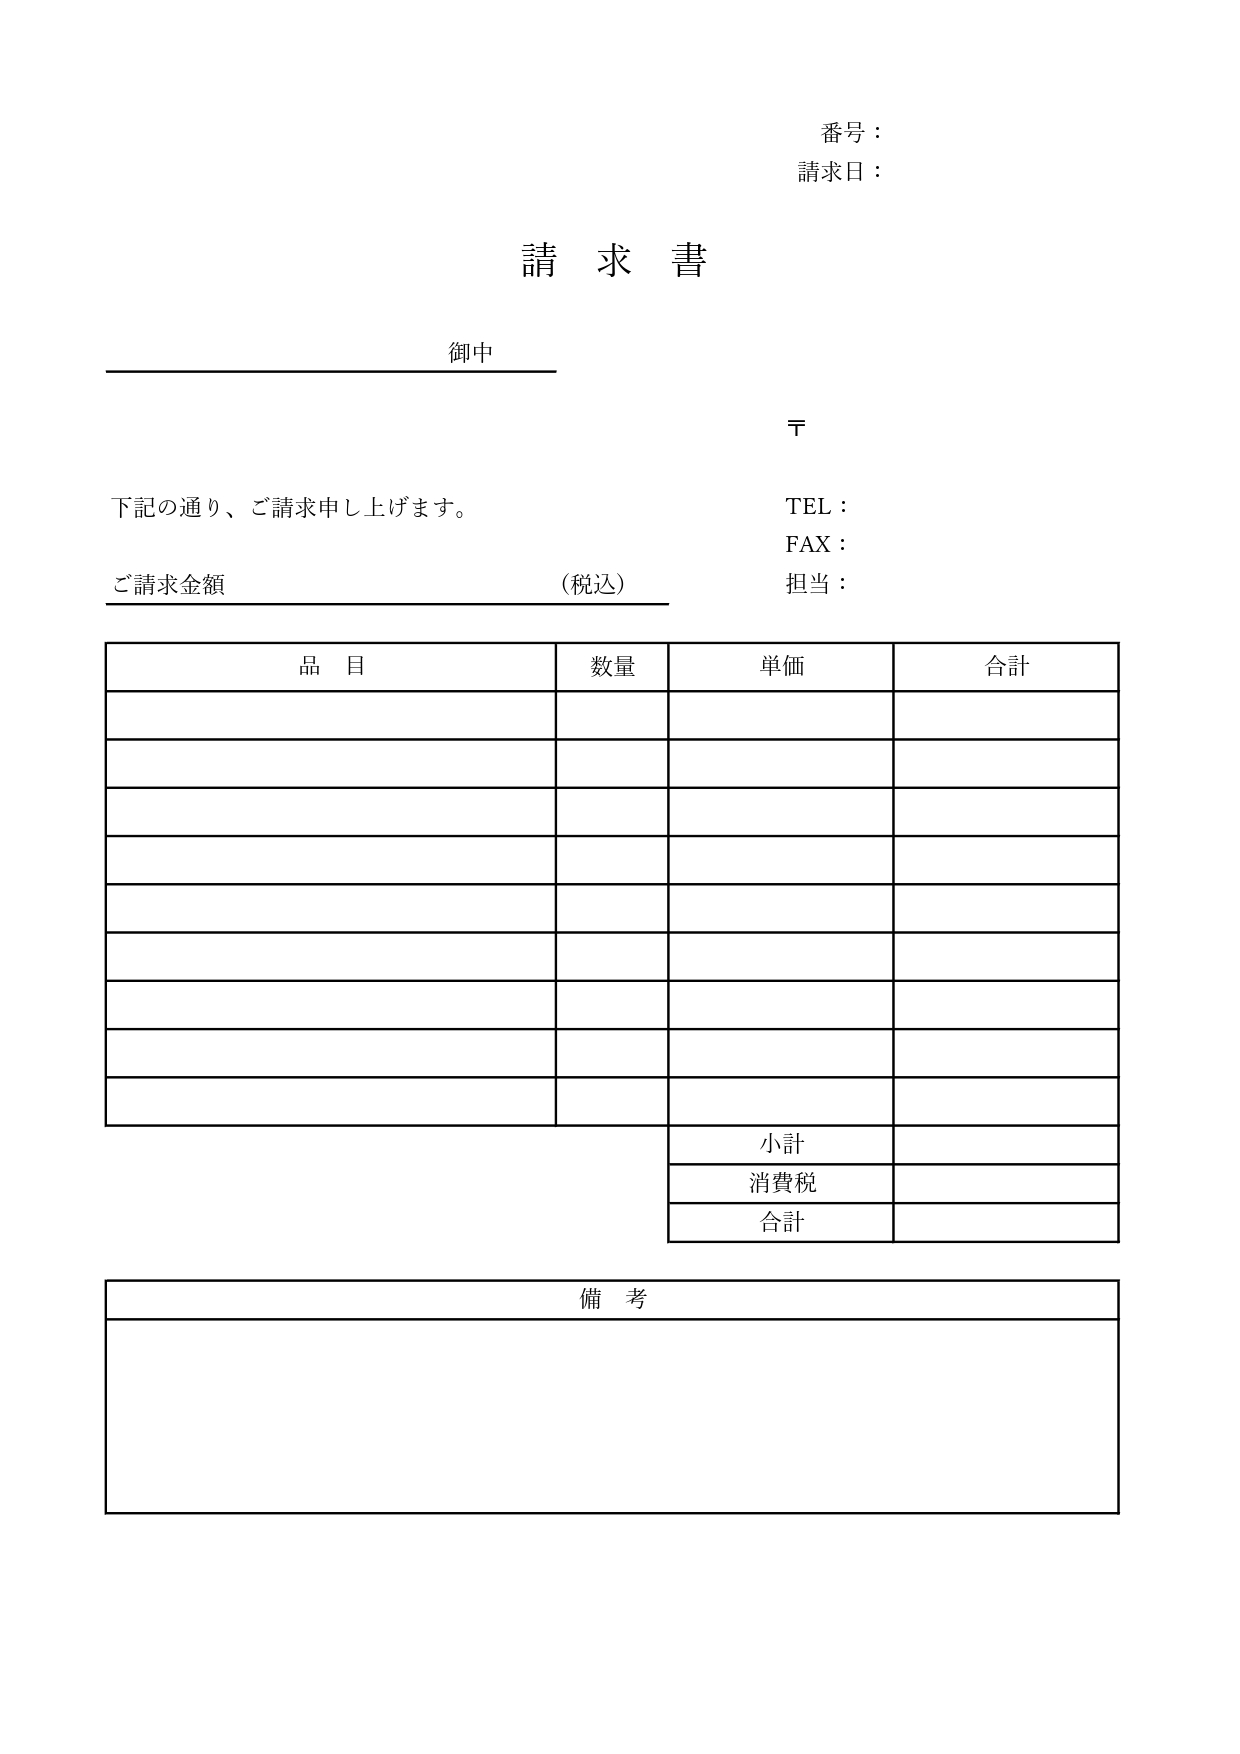
\includegraphics[width=15cm]{image/05-indication/indication_original.jpg}
        }
        \caption{試作したツールを適用する帳票画像}
        \label{fig:indication_original}
    \end{center}
\end{figure}

図\ref{fig:indication_original}に対して、試作したツールを適用し、出力であるJSONファイルと、矩形領域強調画像と下線部領域強調画像の2枚が、実際の矩形領域と下線部領域の位置とラベルがそれぞれ一致することを確認する。
具体的には、矩形領域強調画像と、JSONファイルのrects\_data配列を参照し、矩形領域の出力結果を確認する。
同様に、下線部領域強調画像と、JSONファイル内のunderlines\_data配列を参照し、下線部領域の出力結果を確認する。


\section{矩形領域についての出力結果}\label{sec:result_rect}
本節は、矩形領域についての出力結果を確認する。

図\ref{fig:indication_original}に対して、試作したツールを適用し、出力したJSONファイルのうち、rects\_data配列の一部を、図\ref{fig:rects_data_json}に示す。
図\ref{fig:rects_data_json}のJSONファイルと同時に出力した2枚の領域強調画像のうち、矩形領域を強調した画像の一部を、図\ref{fig:highlighted_rects_part}に示す。

\lstset{language=}
\begin{figure}[t]
    \begin{lstlisting}
        {
            "id": 4,
            "label": "string",
            "coords": {
                "top_left": {
                    "x": 275,
                    "y": 817
                },
                "buttom_left": {
                    "x": 275,
                    "y": 903
                },
                "buttom_right": {
                    "x": 1008,
                    "y": 903
                },
                "top_right": {
                    "x": 1008,
                    "y": 817
                }
            }
        },
        {
            "id": 5,
            "label": "number",
            "coords": {
                "top_left": {
                    "x": 1016,
                    "y": 817
                },
                "buttom_left": {
                    "x": 1016,
                    "y": 903
                },
                "buttom_right": {
                    "x": 1308,
                    "y": 903
                },
                "top_right": {
                    "x": 1308,
                    "y": 817
                }
            }
        },
    \end{lstlisting}
    \caption{rects\_data配列の一部}\label{fig:rects_data_json}
\end{figure}

\begin{figure}[tp]
    \begin{center}
        \fbox{
            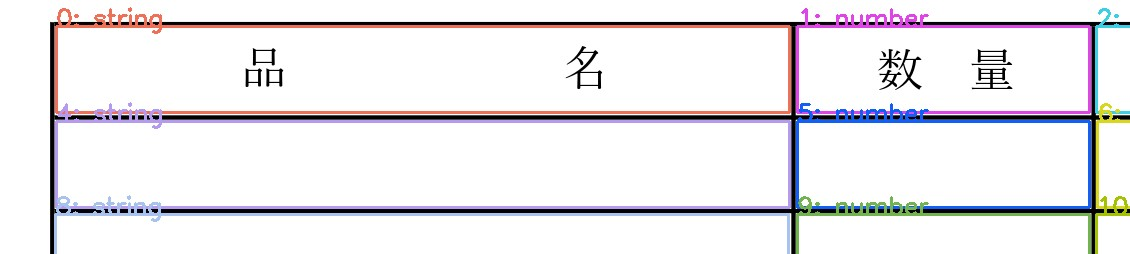
\includegraphics[width=15cm]{image/05-indication/highlighted_rects_part.jpg}
        }
        \caption{矩形領域を強調した画像の一部}
        \label{fig:highlighted_rects_part}
    \end{center}
\end{figure}

矩形領域座標について、IoU(Intersection over Union)を用いて、JSONファイルの出力が正しいことを確認する。

実際の矩形領域座標と、出力するJSONファイルの矩形領域座標を確認し、IoUを算出する。
図\ref{fig:rects_data_json}より、idキーの値が4である矩形領域座標は、左上頂点のxy座標が(275,817)であり、右下頂点のxy座標が(1008,903)である。
図\ref{fig:highlighted_rects_part}にある4番の矩形領域について、図\ref{fig:indication_original}の画像では、左上頂点のxy座標が(273,816)であり、右下頂点のxy座標が(1009,905)であった。
よって、IoUを算出すると、0.96となる。
IoUは、一般に、0.5を閾値として閾値以上である場合は2つの領域が致しているとみなすため、この矩形領域座標は正しく取得できたと言える。
他の矩形領域に対しても、正しく矩形領域座標を取得していることを確認した。

ラベルについては、人間が判断したラベルと、ツールが出力したラベルが一致するかを確認する。
図\ref{fig:rects_data_json}より、idキーの値が4と5である矩形領域について、それぞれのラベルはstringとnumberである。
図\ref{fig:highlighted_rects_part}より、画像内に描画した矩形領域の番号のうち、4番の矩形領域は、「品名」を記入する欄であり、5番の矩形領域は、「数量」を記入する欄であることがわかる。
各矩形領域のラベルについて、「品名」は文字列(string)、「数量」は数値(number)がそれぞれ正しいラベルであるため、これら2つの矩形領域については、正しいラベルを割り付けていることを確認できた。
他の矩形領域に対しても、一部を除き、正しくラベルを割り付けていることを確認した。

また、矩形領域について、JSONファイルと領域強調画像の出力が対応することから、帳票画像のレイアウトを変更せず、矩形領域の領域座標とラベルを出力できたことがわかる。

一部の矩形領域については、本来割り付けるべきラベルとは異なるラベルを誤って割り付けた。
JSONファイルのうち、誤ったラベルを割り付けた矩形領域座標を、図\ref{fig:rects_data_miss_json}に示す。
また、図\ref{fig:rects_data_miss_json}に示した矩形領域座標に対応する矩形領域強調画像を、図\ref{fig:highlighted_rects_miss_part}に示す。

\lstset{language=}
\begin{figure}[t]
    \begin{lstlisting}
        {
            "id": 25,
            "label": "string",
            "coords": {
                "top_left": {
                    "x": 1713,
                    "y": 1283
                },
                "buttom_left": {
                    "x": 1713,
                    "y": 1369
                },
                "buttom_right": {
                    "x": 2262,
                    "y": 1369
                },
                "top_right": {
                    "x": 2262,
                    "y": 1283
                }
            }
        },
    \end{lstlisting}
    \caption{誤ったラベルを割り付けた矩形領域座標}\label{fig:rects_data_miss_json}
\end{figure}

\begin{figure}[tp]
    \begin{center}
        \fbox{
            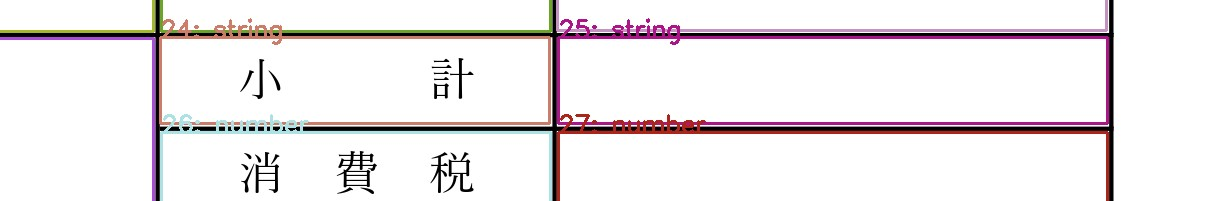
\includegraphics[width=15cm]{image/05-indication/highlighted_rects_miss_part.jpg}
        }
        \caption{図\ref{fig:rects_data_miss_json}の矩形領域を描画した矩形領域強調画像}
        \label{fig:highlighted_rects_miss_part}
    \end{center}
\end{figure}

図\ref{fig:rects_data_miss_json}より、idキーの値が25の矩形領域は、labelキーの値がstringであることがわかる。
図\ref{fig:highlighted_rects_miss_part}より、25番の矩形領域は、「小計」を記入する欄であることがわかる。
本来割り付けるべきラベルは数値(number)であるため、誤ったラベルを割り付けていることがわかる。
これは、「小計」という文字を認識することができなかったことが原因である。

図\ref{fig:indication_original}の画像に対して、認識した文字のバウンディングボックスを描画した画像の一部を、図\ref{fig:OCR_result}に示す。

\begin{figure}[tp]
    \begin{center}
        \fbox{
            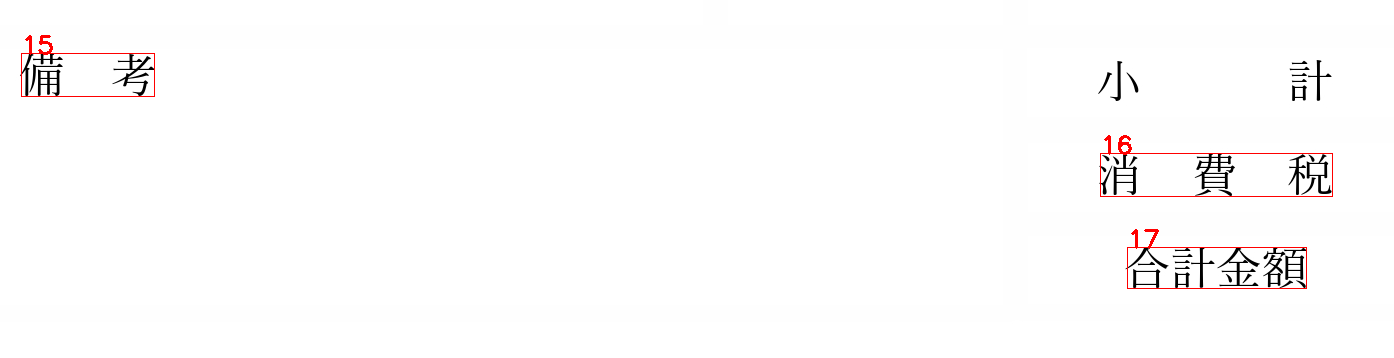
\includegraphics[width=15cm]{image/05-indication/OCR_result.png}
        }
        \caption{図\ref{fig:indication_original}で認識した文字}
        \label{fig:OCR_result}
    \end{center}
\end{figure}

図\ref{fig:OCR_result}の右にある「小計」については、バウンディングボックスを描画していないため、文字認識に失敗していることがわかる。
また、図\ref{fig:OCR_result}の左にある「備考」の文字について、属性を文字列(string)と推測したことを確認した。
このことから、文字認識を失敗したことによって、本来対応する文字とは別の文字の属性をラベルとして割り付けたことが、誤ったラベルを割り付けた原因であることがわかる。
この問題点については、\ref{sec:problems}節で後述する。

\section{下線部領域についての出力結果}\label{sec:result_underline}
本節は、下線部領域についての出力結果を確認する。

図\ref{fig:indication_original}に対して、試作したツールを適用し、出力したJSONファイルのうち、underlines\_data配列の一部を、図\ref{fig:underlines_data_json}に示す。
また、図\ref{fig:underlines_data_json}のJSONファイルと同時に出力した2枚の下線部強調画像のうち、下線部領域を強調した画像の一部を図\ref{fig:highlighted_underlines_part}に示す。

\lstset{language=}
\begin{figure}[t]
    \begin{lstlisting}
        {
            "id": 0,
            "label": "date",
            "left": {
                "x": 869,
                "y": 354
            },
            "right": {
                "x": 1512,
                "y": 354
            }
        },
        {
            "id": 1,
            "label": "number",
            "left": {
                "x": 1908,
                "y": 355
            },
            "right": {
                "x": 2265,
                "y": 355
            }
        },
    \end{lstlisting}
    \caption{underlines\_data配列の一部}\label{fig:underlines_data_json}
\end{figure}

\begin{figure}[tp]
    \begin{center}
        \fbox{
            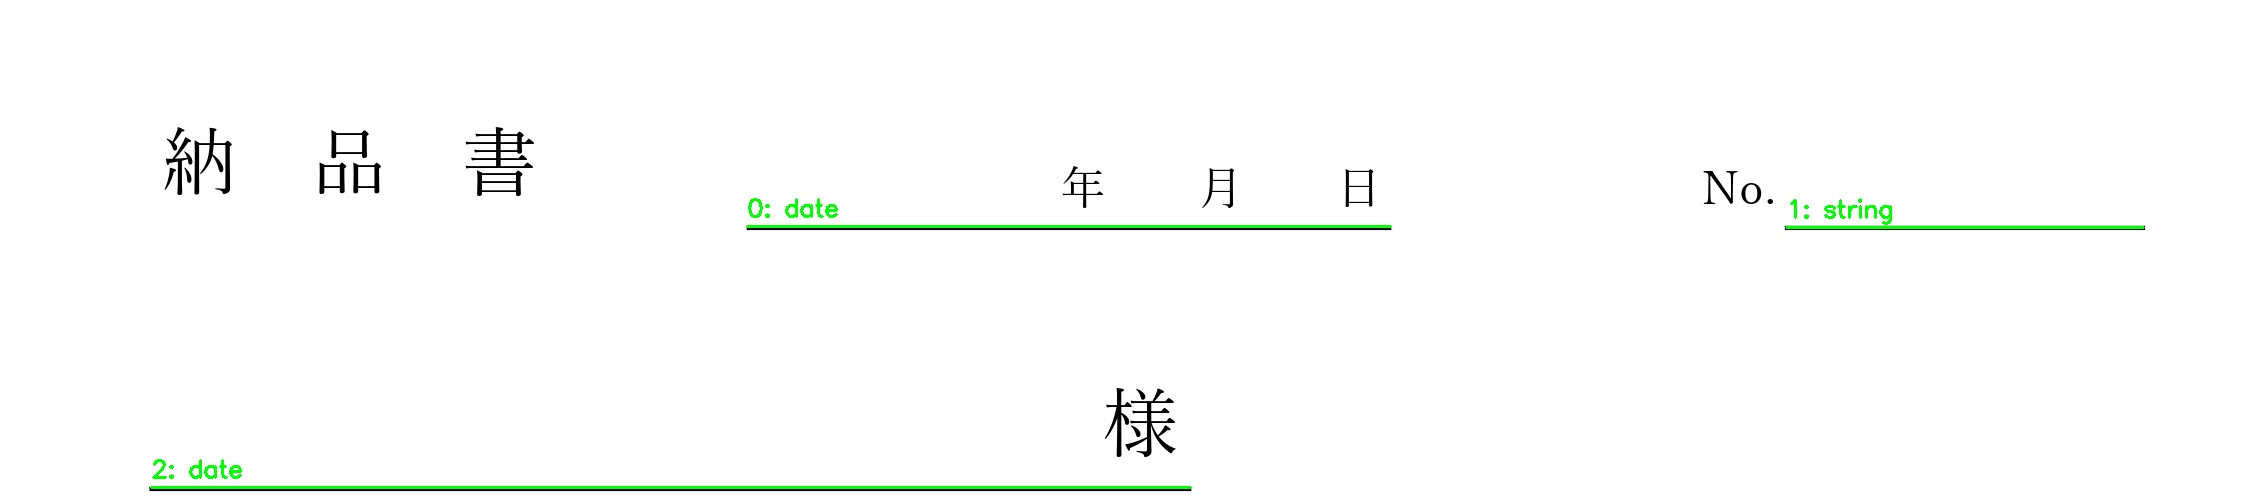
\includegraphics[width=15cm]{image/05-indication/highlighted_underlines_part.jpg}
        }
        \caption{下線部領域を強調した画像の一部}
        \label{fig:highlighted_underlines_part}
    \end{center}
\end{figure}

下線部領域座標については、矩形領域座標と同様に、IoUを用いて、JSONファイルの出力が正しいことを確認する。
なお、下線部領域については、高さを3ピクセルとして、IoUを計算する。
実際の下線部領域座標と、出力するJSONファイルの下線部領域座標を確認し、IoUを算出する。
図\ref{fig:underlines_data_json}より、idキーの値が0である下線部領域座標は、左端点のxy座標が(869,354)であり、右端点のxy座標が(1512,354)である。
図\ref{fig:highlighted_underlines_part}にある0番の下線部領域について、図\ref{fig:indication_original}の画像では、左端点のxy座標が(869,354)であり、右端点のxy座標が(1511,354)であった。
よって、IoUを算出すると、0.99となるため、この下線部領域座標は正しく取得できたと言える。
他の下線部領域に対しても、正しく下線部領域座標を取得していることを確認した。

以降は、下線部領域のラベルについて、出力が正しいことを確認する。
図\ref{fig:underlines_data_json}より、idキーの値は0と1であり、それぞれラベルはdate、numberである。
図\ref{fig:highlighted_underlines_part}より、画像内に描画した矩形領域の番号のうち、0番の下線部領域は、「年月日」を記入する欄であり、1番の下線部領域は、「No.」を記入する欄であることがわかる。
「年月日」は日付(date)、「No.」は数値(number)がそれぞれ正しいラベルであるため、これら2つの下線部領域については、正しいラベルを割り付けていることを確認できた。
他の下線部領域に対しても、一部を除き、正しくラベルを割り付けていることを確認した。

また、下線部領域について、JSONファイルと領域強調画像の出力が対応することから、帳票画像のレイアウトを変更することなく、下線部領域の領域座標とラベルを出力できたことがわかる。

一部の下線部領域については、本来割り付けるべきラベルとは異なるラベルを誤って割り付けた。
JSONファイルのうち、誤ったラベルを割り付けた下線部領域座標を、図\ref{fig:underlines_data_miss_json}に示す。

\lstset{language=}
\begin{figure}[t]
    \begin{lstlisting}
        {
            "id": 2,
            "label": "date",
            "left": {
                "x": 273,
                "y": 615
            },
            "right": {
                "x": 1312,
                "y": 615
            }
        },
    \end{lstlisting}
    \caption{誤ってラベルを割り付けた下線部領域}\label{fig:underlines_data_miss_json}
\end{figure}

図\ref{fig:underlines_data_miss_json}の下線部領域は、図\ref{fig:highlighted_underlines_part}の2番の下線部領域である。
図\ref{fig:underlines_data_miss_json}より、idキーの値が2の下線部領域は、labelキーの値がdateであることがわかる。
図\ref{fig:highlighted_underlines_part}の左下を確認すると、2番の下線部領域は、右にある「様」という文字から、宛名を記入する欄であることがわかる。
本来割り付けるべきラベルは文字列(string)であるため、誤ったラベルを割り付けていることがわかる。
これは、\ref{subsec:label_link_processing}節で述べたラベルを割り付ける手法では、領域座標の右にある文字の属性を参照しないことが原因である。
この問題点については、\ref{sec:problems}節で後述する。
\chapter{考察}\label{cha:Discussion}



\section{本提案手法の有用性に関する評価}\label{sec:evalue_usefulness}

\subsection{記入欄の配置完了までにかかる時間に関する評価}\label{subsec:evalue_required_time}

\subsection{配置した記入欄の精度に関する評価}\label{subsec:evalue_accuracy}
理想は、手作業で配置した精度の100\%に近い精度が提案手法適用時にも出ること。



\section{関連研究}\label{sec:relation_research}



\section{本提案手法の問題点}\label{sec:AWSEL_problems}
\chapter{おわりに}\label{cha:Conclusion}
本研究では、電子フォームの作成にあたって、使い慣れたレイアウトを変更せず、作成に必要な手間と時間を削減することを目的として、帳票画像内における記入欄の領域座標、および、その記入欄に入力する内容のデータ型をまとめたJSONファイルに加えて、検知した記入欄を強調表示した画像2枚を出力する、記入欄の検出およびラベル付与手法を提案した。
本提案手法では、帳票画像を入力として、領域座標とラベルをまとめたJSONファイルと、JSONファイルの内容に対応し、領域とラベルを帳票画像に描画した2枚の領域強調画像を出力とするツールの試作を手段とした。
試作したツールは、以下の2つの機能を持つ。

\begin{itemize}
  \item 領域座標取得およびラベル付与機能\\
      領域座標取得およびラベル付与機能は、帳票画像中の矩形領域および下線部領域について、領域座標を電子フォーム記入欄として取得し、それぞれにラベルを割り付ける機能である。
      ラベルを割り付けることにより、バリデーションチェックに必要な情報を付与することができる。
  \item 領域強調画像出力機能\\
      領域強調画像出力機能は、入力である帳票画像に対して、取得した領域座標とラベルを描画することによって、強調表示したPNG画像を出力する機能である。
      これによって、領域座標取得およびラベル付与機能で出力したJSONファイルの内容を、目視で確認しやすくなる。
      本機能で出力する画像は、矩形領域を強調した矩形領域強調画像と、下線部領域を強調した下線部領域強調画像の計2枚である。
\end{itemize}

適用例を用いて、試作したツールが領域座標の取得と、ラベル割付が一部を除いて正常に動作することを確認した。
なお、正常に動作しない原因は、文字認識が失敗したことによって、想定とは異なるラベルを領域座標に割り付けたことや、記入する内容を示す文字が、帳票画像記入欄の右にあることによって、領域座標の右にある文字の属性を参照しないためであることを確認した。
また、JSONファイルの内容と、2枚の領域強調画像が正しいことと、それらが対応した状態で、帳票画像のレイアウトに忠実に出力することを確認した。

試作したツールの有用性を評価するため、電子フォーム記入欄を配置するまでにかかる時間を計測する実験を行った。
ある帳票画像2枚について、試作したツールを適用することによって、GUIツールのみを用いた場合と比較して、それぞれ平均で4分46秒(約54.17\%)、2分42秒(約37.41\%)短いことから、電子フォーム記入欄を配置するまでにかかる時間を削減できることを確認した。
また、試作ツールの出力について、精度を確認するため、領域座標とラベルの、それぞれの適合率と再現率を評価した。
領域座標およびラベルの再現率は、適合率以上の割合であることから、電子フォーム記入欄の削除による修正回数が、配置による修正回数と比較して多いことが推測できるため、手間を削減できることを確認した。

以上のことから、本研究で提案した手法は、電子フォーム作成にかかる手間と時間の削減に有用であると言える。

今後の課題を、以下に示す。

\begin{itemize}
    \item 記入欄と記入内容を示す欄の区別\\
        特に矩形が隣接する形式の帳票である場合、行や列の先頭に、記入内容を示す矩形の欄があるときがある。
        これにより、帳票画像記入欄ではない矩形の領域座標を不要に取得してしまうため、対応する必要がある。
    \item 領域座標に割り付けるラベルの安定\\
        領域座標に割り付けるラベルは、文字認識と大規模言語モデルの出力に依存する。
        現在のTesseract-OCRでは、文字を100\%正確に認識することができず、大規模言語モデルの出力は実行の度に変化する。
        これにより、電子フォーム記入欄に想定とは異なるラベルを割り付けてしまう場合があるため、対応する必要がある。
    \item レイアウトによる精度の低下\\
        背景や帳票画像記入欄の一部に色が付いている、押印があるなどの二値画像は、黒の画素の数が増加する。
        これにより、帳票画像記入欄の検出やラベル割付の精度が低下してしまう場合があるため、対応する必要がある。
    \item 記入内容を示す文字の判定\\
        ある帳票画像記入欄について、記入する内容を示す文字が右にある場合、ラベルを更新することができない。
        これにより、想定とは異なるラベルを割り付けてしまう場合があるため、対応する必要がある。
    \item 撮影環境による精度の低下\\
        撮影する環境によって、大津の二値化で取得する閾値が変化し、うまく二値化することができない。
        これにより、矩形と下線部を取得できない場合や、文字認識が失敗する場合があるため、対応する必要がある。
\end{itemize}

% \section{はじめに}\label{cha:Introduction}
% \tool 作ったよ。
% 先行研究\cite{example}を参考にしたよ。

% \section{\tool の機能}

% \section{\tool の適用例}
% \tool にソースコード\ref{lst:input-example}を入力した結果を、図\ref{image/sample.png}に示す。
% \begin{figure}[hb]
% \begin{lstlisting}[label={lst:input-example}, caption={入力例}]
% coordinate00,0,0
% coordinate01,1,1
% coordinate02,2,2
% coordinate03,3,3
% \end{lstlisting}
% \end{figure}

% \begin{figure}[hb]
%     \centering
%     
\includegraphics[scale=0.5]{image/sample.png}
%     \caption{\tool の画面}
%     \label{image/sample.png}
% \end{figure}

% \section{\tool の評価}


% \section{まとめ}

% \footnotesize

%%
% 謝辞
%
\acknowledgment
本研究の遂行と、本論文の執筆にあたり、終始熱心なご指導ご鞭撻を賜りました、宮崎大学工学部情報システム工学科の片山徹郎教授に、心より感謝申し上げます。

また、本研究にあたり、多大なお力添えを賜りました、codeless technology株式会社の皆様に、深く感謝申し上げます。

最後に、片山徹郎研究室の皆様に、感謝いたします。

特に教授と先輩方は、研究方針の相談を聞いてくださり、論文の添削も遅い時間までしていただきました。ありがとうございました。

%%
%参考文献
%
\begin{thebibliography}{0}
  \bibitem{帳票}新村出編: 広辞苑 第六版 (普通版), 岩波書店, 2008
  \bibitem{電子文書と電子化文書}株式会社マネーフォワード: "電子文書とは?電子化文書の比較とメリット、注意点を解説!"\\\url{https://biz.moneyforward.com/contract/basic/2035/}\\アクセス日: 2024/01/09.
  \bibitem{OpenCV}OpenCV: "opencv"\\\url{https://github.com/opencv/opencv/blob/master/LICENSE}\\アクセス日: 2024/01/09.
  \bibitem{ガウシアンフィルタ}鳥取大学 OpenCV-Pythonチュートリアル: "画像の平滑化"\\\url{http://labs.eecs.tottori-u.ac.jp/sd/Member/oyamada/OpenCV/html/py_tutorials/py_imgproc/py_filtering/py_filtering.html}\\アクセス日: 2024/01/10.
  \bibitem{大津の二値化}大津展之: "認識問題としての二値化と各種方法の検討", 1980年電子情報通信学会論文誌 Vol.J63-D No.4, pp.349-356, 1980
  \bibitem{画素値}MathWorks: "8ビットと16ビットイメージ"\\\url{https://jp.mathworks.com/help/matlab/creating_plots/working-with-8-bit-and-16-bit-images.html}\\アクセス日: 2024/01/11.
  \bibitem{エッジ検出}LearnOpenCV: "Edge Detection Using OpenCV"\\\url{https://learnopencv.com/edge-detection-using-opencv/}\\アクセス日: 2024/01/10.
  \bibitem{カーネルの作成}OpenCV.jp: "画像フィルタリング — opencv 2.2 documentation"\\\url{http://opencv.jp/opencv-2svn/cpp/image_filtering.html}\\アクセス日: 2024/01/15.
  \bibitem{膨張処理}MathWorks: "モルフォロジー演算のタイプ"\\\url{https://jp.mathworks.com/help/images/morphological-dilation-and-erosion.html}\\アクセス日: 2024/01/10.
  \bibitem{Canny法}鳥取大学 OpenCV-Pythonチュートリアル: "Canny法によるエッジ検出"\\\url{http://labs.eecs.tottori-u.ac.jp/sd/Member/oyamada/OpenCV/html/py_tutorials/py_imgproc/py_canny/py_canny.html}\\アクセス日: 2024/01/10.
  \bibitem{輪郭検出}鳥取大学 OpenCV-Pythonチュートリアル: "輪郭: 初めの一歩"\\\url{http://labs.eecs.tottori-u.ac.jp/sd/Member/oyamada/OpenCV/html/py_tutorials/py_imgproc/py_contours/py_contours_begin/py_contours_begin.html#contours-getting-started}\\アクセス日: 2024/01/28.
  \bibitem{ハフ変換}MathWorks: "ハフ変換"\\\url{https://jp.mathworks.com/discovery/image-transform.html}\\アクセス日: 2024/01/28.
  \bibitem{HoughLinesP関数の引数}OpenCV: "Feature Detection"\\\url{https://docs.opencv.org/3.4/dd/d1a/group__imgproc__feature.html#ga8618180a5948286384e3b7ca02f6feeb}\\アクセス日: 2024/01/28.
  \bibitem{輪郭描画}OpenCV: "OpenCV: Contours : Getting Started"\\\url{https://docs.opencv.org/3.4/d4/d73/tutorial_py_contours_begin.html}\\アクセス日: 2024/01/28.
  \bibitem{DeblurGANv2}Orest Kupyn and Tetiana Martyniuk and Junru Wu and Zhangyang Wang: "DeblurGAN-v2: Deblurring (Orders-of-Magnitude) Faster and Better", The IEEE International Conference on Computer Vision (ICCV), pp.8878-8887, 2019
  \bibitem{DeblurGANv2の先行研究}Emilda Zhang,  Vincent Ardyan Putra, and Gede Putra Kusuma: "Improving optical character recognition accuracy for Indonesia identification card using generative adversarial network", Journal of Theoretical and Applied Information Technology Vol.100 No.8, pp.2424-2437, 2022
  \bibitem{光学文字認識}比留川翔哉, 丸山一貴: "本の厚みによる歪みを考慮した光学文字認識", 情報処理学会 第60回プログラミング・シンポジウム, pp.81-86, 2019
  \bibitem{Fugashi}McCann, Paul: "fugashi, a Tool for Tokenizing Japanese in Python", Proceedings of Second Workshop for NLP Open Source Software (NLP-OSS), pp.44-51, 2020
  \bibitem{UniDic品詞体系}言語資源開発センター: 伝康晴, 山田篤, 小椋秀樹, 小磯花絵, 小木曽智信: "UniDic version 1.3.9 ユーザーズマニュアル"\\\url{https://clrd.ninjal.ac.jp/unidic/UNIDIC_manual.pdf}\\アクセス日: 2024/01/09.
  \bibitem{Youri}rinna: "rinna、Llama 2の日本語継続事前学習モデル「Youri 7B」を公開"\\\url{https://rinna.co.jp/news/2023/10/20231031.html}\\アクセス日: 2024/01/09.
\end{thebibliography}

% \newpage
% \listoftodos
\end{document}
